% !TeX root = ../main.tex

\chapter{龙芯安卓图形栈设计与实现}
本章将详细介绍在现有龙芯硬件平台下,安卓图形栈的设计与实现。首先是对图形系统进行分析,从整体架构上介绍图形系统的基本框架,包括安卓框架部分以及龙芯硬件
支持部分,以及如何在Android上支持LoongArch和LG110。之后介绍图形系统的四个主要组成部分:内核图形驱动模块,用户态图形驱动模块,安卓gralloc模块和硬件混合渲染(HWC)模块。内核驱动模块负责对接用户态驱动
和GPU固件之间的联系。用户态驱动负责向安卓框架提供龙芯硬件支持。而gralloc模块是根据龙芯硬件驱动向安卓上层libui库提供服务,硬件混合渲染(HWC)模块为安卓中进行窗口
(Layer)合成和显示的HAL模块。(标注:还需完善,暂且这样)

\section{系统需求分析}

首先对图形系统的关键服务SurfaceFlinger进行分析,分析龙芯显卡需要对图形系统中的哪些组件进行支持,再分析这些组件的需求。

\subsection{SurfaceFlinger关键服务分析}
Android图形系统作为移动端计算机的核心子系统,构建了从应用程序界面到物理显示设备的完整视觉呈现管道。
这个复杂的系统包含超过50个核心组件,其中SurfaceFlinger作为系统级的合成引擎,承担着最核心的图形处理任务。
整个系统的运作可以分解为三个层次架构:应用层、图形处理层和硬件抽象层。
应用层负责通过UI框架构建图形界面元素,图形处理层包括渲染引擎和合成器引擎,硬件抽象层主要是为这两个引擎提供支持。

渲染引擎分析:渲染引擎​是负责将抽象的图形描述转化为最终可视像素的软件系统。Android渲染引擎默认使用的是skia,
在SurfaceFlinger初始化过程中,会创建一个线程专门用于skia引擎的初始化并用于后续的图形绘制,
在SkiaGLRenderEngine::create时,会依次执行eglGetDisplay获取EGL显示句柄,此句柄代表了要渲染的物理设备;eglInitialize初始化EGL环境,并获得EGL的主次版本号;
eglQueryString查询与当前显示连接相关的字符串信息,包括EGL版本信息、供应商版本信息以及支持的客户端API等,安卓还会使用EGL\_EXTENSIONS
获取有关安卓特性的拓展并初始化;使用createEglContext在EGL中创建 OpenGL ES 上下文;然后使用eglMakeCurrent将指定的渲染上下文和表面设置为当前的函数。
因此渲染引擎的正常运行需要OpenGL ES相关实现支持。

合成器引擎分析:SurfaceFlinger中集成了合成器引擎CompositionEngine,也是SurfaceFlinger的核心部分,负责将多个图层按照z轴顺序合成并渲染等。
其作为硬件混合渲染器的客户端,会通过跨进程通信的方式调用框架中的Icomposer实现和接口,从而完成与具体硬件混合渲染器的交互。因此合成器引擎需要硬件混合渲染器实现的支持。
而合成器在合成图像时需要向系统申请图形缓存,因此也需要图形内存缓存分配的实现。

由上,为了实现对SurfaceFlinger的支持,需要OpengGL ES实现、硬件抽象层需要完成gralloc和HWC服务。 

\subsection{安卓硬件驱动接口需求}
由上节关键服务分析可知,需要在安卓硬件抽象层实现gralloc和HWC服务。而安卓对硬件抽象层服务有着完成的规范和接口限制,具体需要严格按照相应的接口实现。
自Android Q版本开始,为了提供图形性能和增强对硬件的支持,对图形系统进行了重构与优化,至S版本稳定下来,中间迭代了4个API版本,
具体表现为,引入了Gralloc2 API(至Android S版本Gralloc4稳定)和HWC2,本课题基于gralloc4以及composer2.1实现。
gralloc模块需要完成内存分配、缓冲区映射、缓冲区管理、性能优化等多方面的功能,hwcomposer模块则需要实现图层管理、显示输出、合成控制、与gralloc适应相关的功能。
gralloc模块HAL接口分别定义在/hardware/interfaces/graphics/allocator和/hardware/interfaces/graphics/mapper下,
其中HAL接口表统计如表\ref{tab:gralloc模块HAL接口}。而HWC模块的实现较为复杂,包含服务端和客户端,服务端的实现集中在/hardware/interfaces/graphics/composer下,
通过调用硬件供应商的具体实现共同组成服务端,客户端是指如SurfaceFlinger中的CompositionEngine通过跨进程调用服务端的实现。
在考虑到目前龙芯硬件平台并没有支持HWC的硬件,因此仅需要保证hwcomposer的client合成模式功能,也就是使用GPU合成图层并写入缓冲区的功能。

\begin{table}[h]
  \centering
  \caption{gralloc模块HAL接口}
  \label{tab:gralloc模块HAL接口}
  \begin{tabular}{llll}
    \toprule
    接口  & 组 & 接口 & 组\\
    \midrule
    createDescriptor & IMapper & get & IMapper \\
    importBuffer & IMapper & set & IMapper\\
    freeBuffer & IMapper & getFromBufferDescriptorInfo & IMapper\\
    validateBufferSize & IMapper & listSupportedMetadataTypes & IMapper\\
    getTransportSize & IMapper & dumpBuffer  & IMapper\\
    lock & IMapper & getReservedRegion & IMapper\\
    unlock & IIMapper & allocate & IAllocator\\
    flushLockedBuffer & IMapper & isSupported & IMapper\\
    rereadLockedBuffer & IMapper \\
    \bottomrule
  \end{tabular}
  \note{}
\end{table}

\subsection{兼容性需求}
由于安卓是一个开源项目,因此任何硬件制造商都可以制造搭载安卓操作系统的设备,但兼容安卓的前提是可以正常运行安卓的执行环境和应用。
根据Android12的兼容性文档\cite{Android-12-cdd}中有关2D和3D图形加速的部分,对于显卡和配套驱动作出如下约束,必须支持OpenGL ES 1.1和2.0,
以及如下10种拓展\ref{tab:Android12兼容拓展要求}。目前龙芯LG110及配套已满足相关兼容性标准。

\begin{table}[h]
  \centering
  \caption{Android12兼容拓展要求}
  \label{tab:Android12兼容拓展要求}
  \begin{tabular}{l}
    \toprule
    拓展名  \\
    \midrule
    EGL\_KHR\_image \\
    EGL\_KHR\_image\_base \\
    EGL\_ANDROID\_image\_native\_buffer \\
    EGL\_ANDROID\_get\_native\_client\_buffer \\
    EGL\_KHR\_wait\_sync \\
    EGL\_KHR\_get\_all\_proc\_addresses \\
    EGL\_ANDROID\_presentation\_time \\
    EGL\_KHR\_swap\_buffers\_with\_damage \\
    EGL\_ANDROID\_recordable \\
    EGL\_ANDROID\_GLES\_layers \\
    \bottomrule
  \end{tabular}
  \note{}
\end{table}

\subsection{架构差异分析}
\label{sec:架构差异分析}
本课题需要在LoongArch架构下实现,而Android多应用于ARM架构,ARM与LoongArch架构的图形系统有较大差异,具体表现为ARM架构下的GPU没有独立显存\cite{Inki},
而在LoongArch的内核中,是使用DRI框架来调用GPU,并且GPU有自己的独立显存。
对LG110内存模型进行分析,LG110内存架构采用分层设计\ref{fig:LG110内存模型},包含GPU本地VRAM和系统主存中的GTT内存模块。
其实现原理体现为:GPU的VRAM通过PCI总线直接映射至CPU的地址空间,允许CPU通过标准PCIe协议直接访问这部分显存资源;
而GTT内存作为动态管理区域,借助页表机制将系统物理内存映射到虚拟地址空间,需经MMU转换后才能被访问。
就GPU端的数据访问逻辑而言,其采用分级的页表管理策略。针对本地VRAM区域,页表项直接记录该存储块的物理地址,使得GPU可直接基于物理地址进行存取操作;
而对于映射至系统主存的GTT区域,页表项存储的是经过DMA引擎转换后的设备地址,因此可以根据DMA的地址发起 DMA 请求获取数据。

\begin{figure}
  \centering
  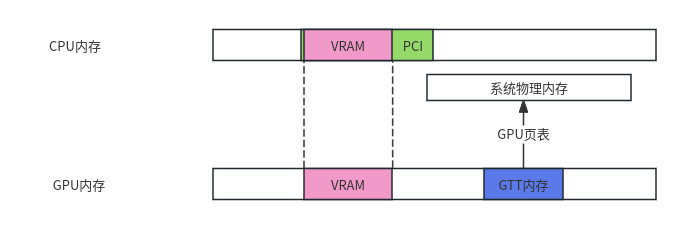
\includegraphics[width=0.8\textwidth]{LG110内存模型.jpg}
  \caption{LG110内存模型}
  \label{fig:LG110内存模型}
\end{figure}

因此,首先需要解决的是在LoongArch架构下,Android系统中显存和系统内存分配映射的问题。AndroidX86\cite{AndroidX86}
很大程度上解决这个问题,该项目使用Mesa作为OpenGL ES实现,基于DRM和GEM实现了gralloc模块,成功的在x86架构下运行SurfaceFlinger并实现硬件加速\cite{XTYY201710015}。
基于这个思路,我们也可以使用Mesa作为OpenGL ES实现以及mesa提供的GBM(General Buffer Manager)来管理缓冲区,为此需要LoongArch架构的DRM框架和用户态libdrm的支持。
其中DRM框架需要基于安卓通用内核5.10实现。
% \subsubsection{安卓硬件驱动接口需求}
% 2.更多特性支持
% \subsection{非功能性需求} 
% 1.兼容性
% 2.高效性
% 3.快速启动

\section{图形系统整体设计}
经过上节需求分析,课题为系统设计了基于龙芯显卡LG110的安卓图形系统方案。本节将对系统整体做一个概述。

\begin{figure}[h]
  \centering
  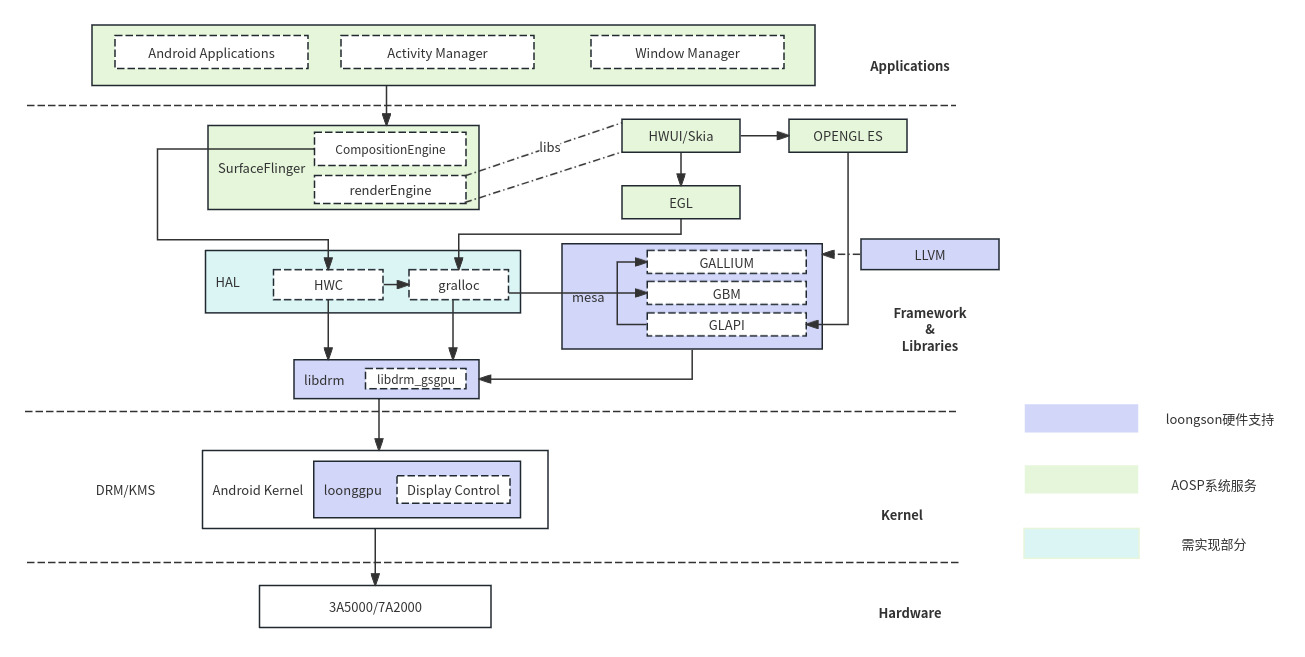
\includegraphics[width=1\textwidth]{图形栈总体结构图.jpg}
  \caption{图形栈总体结构图}    
  \label{fig:图形栈总体结构图}
\end{figure}

自上往下分析,Android应用(Android Applications)、活动管理器(Activity Manager)、窗口管理器(Window Manager)以及部分安卓Native程序(如BootAnimation)
等首先与Surface进行交互,根据自己的需求创建一个Surface,然后数个Surface会被SurfaceFlinger进行混合\cite{邓凡平2011深入理解}。
因此图形系统中最关键的服务进程就是SurfaceFlinger,负责管理图形缓冲区的合成与显示,如图\ref{fig:图形栈总体结构图}所示,它将来自不同应用的图形缓冲区进行合成,
并将合成结果发送到显示设备。SurafaceFlinger包含两个主要引擎合成引擎CompositionEngine和渲染引擎renderEngine,其中renderEngine在Android Q版本时被移至libs下作为相对独立的模块,
但仍然是SurfaceFlinger功能重要组成部分。CompositionEngine是作为HWC的客户端通过IPC方式调用HAL中HWC实现,而renderEngine主要是skia渲染引擎,该引擎通过EGL和OpenGL ES实现
3D硬件加速,需要HAL的gralloc和显卡OpenGL ES实现的支持。因此,图形系统的正确运行一个重要的环节就是确保SurfaceFlinger的正确运行。

而由上文可知,SurfaceFlinger的运行依赖于硬件抽象层和底层图形库。这其中有两个重要的模块,一个是HWC(硬件混合渲染器),是进行窗口合成和显示HAL层模块,其实现是特定于设备的,
通常是由显示设备制造商完成。其用于合成从Surfaceflinger接收的图层,从而减少GPU执行的合成量。
但是实际上由于LG110并不是专门为安卓平台设计的显卡,并没有实现硬件图层混合的功能,因此hwcomposer使用的是client合成模式,
也就是直接使用GPU的OpenGL ES实现进行合成。另一个模块是gralloc。它是Android中负责申请和释放GraphicBuffer的HAL层模块,
由硬件驱动提供实现,为BufferQueue机制提供了基础。gralloc的主要组件包括Allocator,Mapper。Allocator 负责内存的分配和释放,
主要功能包括:根据请求的大小和格式分配内存缓冲区,负责跟踪已分配和空闲的内存块以及支持在多个进程之间共享缓冲区,使得不同的应用程序或组件能够访问同一块内存。
Mapper负责将已分配的缓冲区映射到进程的虚拟地址空间。本课题需要实现支持龙芯硬件平台的gralloc和HWC模块的库以支持SurfaceFlinger的正确运行,即\ref{fig:图形栈总体结构图}中
需实现部分标注。

龙芯显卡驱动栈的方案,采用了mesa作为用户态驱动提供OpenGL ES实现和GBM加上DRM显示框架的方案。
安卓的framework层以及库函数依赖的图形接口是由libdrm进行封装,包括上文提及的gralloc和HWC都是需要使用libdrm定义的接口。
libdrm是一个用户态空间的库,提供了与 Linux 内核中的 DRM子系统交互的接口。它是 Linux 图形栈的核心组件之一(同样也是Android图形栈的方案),
通过封装 DRM 的 IOCTL 系统调用,为用户空间程序提供了简单易用的 API。
至于内核部分仍然是依赖linux内核的KMS和DRM。DRM/KMS 是 Linux 内核中用于管理图形硬件的子系统,提供了对 GPU、显示控制器和显示设备的统一抽象。在上层的系统级服务中,
SurfaceFlinger是通过HWC(Hardware Composer)与DRM/KMS交互,HWC负责将图形缓冲区合成任务委托给硬件。在 DRM/KMS 框架下,HWC 通过 DRM 接口与内核通信,
管理显示模式设置、缓冲区分配和显示同步等任务。KMS 负责配置显示控制器和显示设备的分辨率、刷新率等参数,而 DRM 则管理图形缓冲区的分配与渲染。
OpenGL ES的实现是由用户态驱动mesa提供,而mesa实现的OpenGL ES接口在已有的X图形协议上已有过相关测试。


% 由于loongnix上测试内核版本为4.19,而本次课题采用的内核版本为5.10。
% 由于内核DRM模块的变化较多,因此在原有的4.19的驱动栈基础上,需要实现5.10的驱动栈。该方案并不涉及图形编程接口即OpenGL ES的实现,而主要集中于图形缓冲区的分配上,在后续章节会说明相关变化。
% 因此在\ref{fig:图形栈总体结构图}上标注loongson硬件支持表示需要进行一定的版本适配。

在后续章节中,将从驱动内核模块、用户态驱动、Android HAL层实现以及系统镜像定制等4个部分说明方案。


% 下面以eglInitialize为例,说明surfaceflinger是如何通过安卓的framework层的接口调用龙芯用户态驱动程序的。

% 首先是surfaceflinger初始化,调用flinger->init函数,根据PROPERTY\_DEBUG\_RENDERENGINE\_BACKEND宏判断使用渲染引擎的类型,可以是GLESRenderEngine
% 或SkiaGLRenderEngine,安卓中一般默认的都是SkiaGLRenderEngine,然后是引擎的create。调用eglInitialize,会使用LayerLoader::LoadLayers
% 中dlopen加载的libGLES\_mesa.so去初始化修饰的egl\_connection\_t结构体,调用gEGLImpl的接口,从而实现对龙芯用户态显卡驱动的调用。
% GPU驱动的加载在Surfaceflinger的初始化过程中skia创建时进行加载,根据设置的驱动加载方式(本文使用的是dri2)
% 在eglInitialize时通过eglApi的接口调用mesa中的eglInitialize函数dri2\_initialize,从而实现mesa驱动的加载和初始化。

\section{GPU驱动内核模块的实现}
现代操作系统对硬件资源的管理存在两种典型的设计模式:
1.直接访问模式​(如 MS-DOS):允许用户程序绕过内核直接操作硬件设备,通过物理地址空间或专用 I/O 端口实现低级控制
2.抽象隔离模式​(如 Linux):内核通过硬件抽象层(HAL)屏蔽物理设备细节,所有硬件操作必须通过标准化的系统调用(如 open(), ioctl())发起,内核负责资源调度和安全审查。
驱动程序就是操作系统内核和硬件沟通的桥梁,准确来说就是内核的一部分。

\subsection{IOCTL命令码设计}
在内核驱动程序中,除了基本的设备读写操作(即读取和写入数据)外,设备驱动程序还需要支持对设备执行各种控制操作。
这些控制操作通常是通过 ioctl(Input/Output Control)机制来实现的,它提供了一种用户空间和内核空间之间进行特定设备操作交互的方式。
IOCTL 可以用于实现设备驱动的各种功能,包括配置设备、读取设备状态、传输数据、控制设备行为等,而这些具体的功能需要在驱动程序中实现。
本课题的GPU驱动模块是基于DRM框架,而DRM框架下核心系统调用入口函数ioctl实现的函数原型为

long drm\_ioctl(struct file *filp,unsigned int cmd, unsigned long arg)

其中filp是用户空间传递的文件描述符,表示打开的 DRM 设备文件的上下文,cmd 是用户空间传入的 IOCTL 命令标识符,一般是提前定义好的操作码,与内核驱动中具体的操作函数相对应。
args 是以unsigned long类型传递的,是用户空间传递的命令参数,可能是整数值或者是结构体指针。

因此要实现IOCTL首先需要设计选择ioctl命令码。在linux内核中,ioctl的命令码的结构是一个32位的整数,由四个部分组成,从高位往低位依次是\ref{tab:ioctl命令码结构}:
方向位,占用命令码的第 ​31-30 位​,标识命令的数据传输方向,可能的值有\_IOC\_NONE(无数据)、\_IOC\_READ(内核读)、\_IOC\_WRITE(内核写)、\_IOC\_READ|\_IOC\_WRITE(双向数据);
类型,又称幻数,占用命令码的第 ​24-27 位,用于标识命令所属的设备或子系统,防止命令冲突,通常会选择一个ASCII 字符,确保不同驱动间的幻数不重复,本文由于涉及到的是drm模块所以是d。
同时幻数定义需要在内核驱动和用户空间如libdrm中头文件保持一致;
序号,占用命令码的第 ​16-23 位,在同一幻数下唯一标识具体命令;
数据大小占用命令码的第 ​0-15 位,是ioctl操作涉及的数据结构大小(以字节为单位),仅会对\_IOW、\_IOR、\_IOWR命令有效。
综合各字段,完整的命令码计算方式为:

cmd = (direction << 30) | (magic << 24) | (number << 16) | (size \& 0xFFFF)

在linux内核中还定义了几个辅助宏用于生成具体的命令码,如图\ref{fig:IOCTL辅助宏定义}。

\begin{table}[h]
  \centering
  \caption{ioctl命令码结构}
  \label{tab:ioctl命令码结构}
  \begin{tabular}{llll}
    \toprule
    方向  & 类型 & 序号 & 数据大小 \\
    \midrule
    2bit & 8bit & 8bit & 14bit \\
    \bottomrule
  \end{tabular}
  \note{}
\end{table}

\begin{figure}[h]
  \centering
  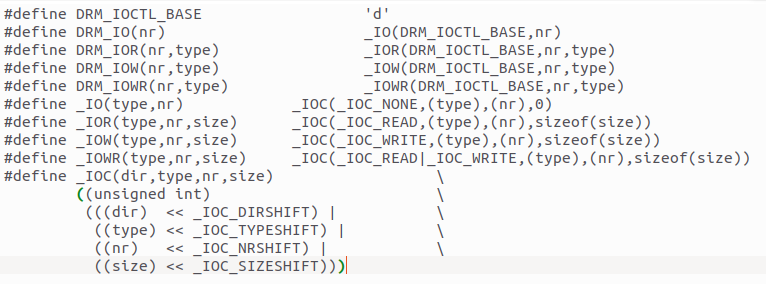
\includegraphics[width=0.8\textwidth]{IOCTL辅助宏定义.png}
  \caption{IOCTL辅助宏定义}
  \label{fig:IOCTL辅助宏定义}
\end{figure}

在课题场景下,需要将内核调用的结果返回,因此使用双向的数据传输作为基础,实现GSGPU的ioctl。
为了给用户态程序提供创建和管理 GEM(图形内存对象)到处理上下文、命令流、内存映射、调度等支持,定义了如表\ref{tab:IOCTL命令码表}ioctl命令码。

\begin{table}[h]  
  \centering
  \caption{IOCTL命令码表}
  \label{tab:IOCTL命令码表}
  \resizebox{\linewidth}{!}{
  \begin{tabular}{llll}
    \toprule
    序号​	&​ 命令​ &​ 功能领域​	& 映射函数 \\
    \midrule
    0x00	& DRM\_GSGPU\_GEM\_CREATE	& ​GEM 内存管理​ & gsgpu\_gem\_create\_ioctl \\
    0x01	& DRM\_GSGPU\_GEM\_MMAP	& ​内存映射​ & gsgpu\_gem\_mmap\_ioctl \\
    0x02	& DRM\_GSGPU\_CTX	& ​上下文管理​	& gsgpu\_ctx\_ioctl\\
    0x03	& DRM\_GSGPU\_BO\_LIST	& ​缓冲区对象列表​	& gsgpu\_bo\_list\_ioctl\\
    0x04	& DRM\_GSGPU\_CS	& ​命令流控制​	& gsgpu\_cs\_ioctl\\
    0x05	& DRM\_GSGPU\_INFO	& ​设备信息查询​	& gsgpu\_info\_ioctl\\
    0x06	& DRM\_GSGPU\_GEM\_METADATA	& ​元数据管理​	& gsgpu\_gem\_metadata\_ioctl\\
    0x07	& DRM\_GSGPU\_GEM\_WAIT\_IDLE	& ​同步与闲置状态​	& gsgpu\_gem\_wait\_idle\_ioctl\\
    0x08	& DRM\_GSGPU\_GEM\_VA	& ​虚拟地址分配​	& gsgpu\_gem\_va\_ioctl\\
    0x09	& DRM\_GSGPU\_WAIT\_CS	& ​命令流同步​	& gsgpu\_cs\_wait\_ioctl\\
    0x10	& DRM\_GSGPU\_GEM\_OP	& ​通用 GEM 操作​	& gsgpu\_gem\_op\_ioctl\\
    0x11	& DRM\_GSGPU\_GEM\_USERPTR	& ​用户指针支持​	& gsgpu\_gem\_userptr\_ioctl\\
    0x12	& DRM\_GSGPU\_WAIT\_FENCES	& ​栅栏同步​	& gsgpu\_cs\_wait\_fences\_ioctl\\
    0x13	& DRM\_GSGPU\_VM	& ​虚拟内存管理​	& gsgpu\_vm\_ioctl\\
    0x14	& DRM\_GSGPU\_FENCE\_TO\_HANDLE	& ​栅栏与句柄映射​	& gsgpu\_cs\_fence\_to\_handle\_ioctl\\
    0x15	& DRM\_GSGPU\_SCHED	& ​任务调度​	& gsgpu\_sched\_ioctl\\
    0x16	& DRM\_GSGPU\_HWSEMA\_OP	& ​硬件信号量操作​	& gsgpu\_hw\_sema\_op\_ioctl\\
    \bottomrule
    \end{tabular}
  }
  \note{}
\end{table}

\begin{enumerate}[1)]
  \item GSGPU\_GEM\_CREATE:在内核中为GPU设备分配并初始化一个GEM对象。
  \item GSGPU\_GEM\_MMAP:将GEM对象映射到用户空间,允许用户态直接访问显存。
  \item GSGPU\_CTX:创建/销毁GPU上下文,管理上下文资源。
  \item GSGPU\_BO\_LIST:管理一组缓冲区对象操作的集合,用于批量操作。
  \item GSGPU\_CS:提交命令流到GPU硬件执行。
  \item GSGPU\_INFO:查询GPU硬件参数
  \item GSGPU\_GEM\_METADATA:设置/获取GEM对象的元数据,主要用于tiling模式或者缓存策略的选择。
  \item GSGPU\_GEM\_WAIT\_IDLE:等待GEM对象关联的所有GPU操作完成。
  \item GSGPU\_GEM\_VA:管理GEM对象的虚拟地址绑定,控制GPU虚拟地址空间映射。
  \item GSGPU\_WAIT\_CS:等待指定命令流完成执行。
  \item GSGPU\_GEM\_OP:对GEM对象执行通用操作,包括创建信息、设置内存放置域等。
  \item GSGPU\_GEM\_USERPTR:通过用户态指针注册内存作为GEM对象,支持零拷贝数据传输。
  \item GSGPU\_WAIT\_FENCES:等待多个栅栏信号完成。
  \item GSGPU\_VM:GPU 虚拟化管理的基础接口。
  \item GSGPU\_FENCE\_TO\_HANDLE:将栅栏转换为句柄,支持跨进程同步。
  \item GSGPU\_SCHED:配置调度策略,更改命令流执行顺序。
  \item GSGPU\_HWSEMA\_OP:操作硬件信号量,控制硬件级资源争用。
\end{enumerate}
由于这些功能大部分需要双向数据传输,所以大部分的命令码使用辅助宏DRM\_IOWR,可以用公式表示为:

\#define DRM\_IOCTL\_ioctl

 DRM\_IOWR(DRM\_COMMAND\_BASE+DRM\_ioctl,union structIoctl)

其中ioctl对应某个命令码,以DRM\_GSGPU\_GEM\_CREATE为例,ioctl=GSGPU\_GEM\_CREATE,structIoctl表示该命令码对应的数据大小,
DRM\_IOCTL\_ioctl实际上就是经过DRM\_COMMAND\_BASE基地址偏移的命令码。
每个命令码都对应具体的函数实现,通过DRM系统提供的DRM\_IOCTL\_DEF\_DRV宏完成联系。
这个宏的作用是将驱动私有的 IOCTL 命令注册到 DRM 的统一命令表中,并关联对应的处理函数和权限标志。如图\ref{fig:ioctl def drv}。
这里实际上将DRM命令、处理该命令的内核函数指针、权限标志和命令的字符串名称分别存入cmd、func、flags和name域,在内核模块进行PCI设备注册时,
将命令表封装进drm\_device结构体的数据中,并在用户态程序进行ioctl系统调用时根据DRM命令码调用对应的内核函数func实现。
DRM命令码与内核处理函数func的映射关系已在表\ref{tab:IOCTL命令码表}中展示。

\begin{figure}[h]
  \centering
  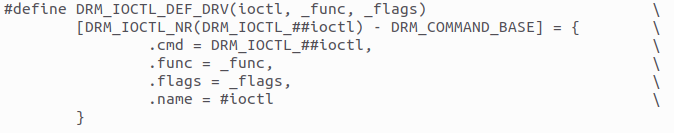
\includegraphics[width=0.8\textwidth]{ioctl def drv.png}
  \caption{DRM\_IOCTL\_DEF\_DRV宏实现}
  \label{fig:ioctl def drv}
\end{figure}

\subsection{内存管理模块}

LG110的内存模型在小节\ref{sec:架构差异分析}和图\ref{fig:LG110内存模型}中已有相关说明。
模块主要功能是管理GPU显存资源(GEM对象)的创建、映射、元数据操作及虚拟地址绑定等。
其主要依赖GEM和TTM对缓冲区对象进行管理。
GEM是内核中用于图形缓冲区管理的一个核心模块,特别是在与图形硬件(如 GPU)交互时。
它是 DRM的一部分,旨在为图形硬件分配、管理和共享内存资源。GEM 的设计目的是简化内存管理,确保图形缓冲区的高效分配和使用,并且能够支持多种类型的设备和硬件架构。
GEM 主要通过图形缓冲区的对象(drm\_gem\_object)来管理 GPU 和显示硬件之间的内存。TTM(Translation Table Manager)适用于GPU内存管理的一部分,
提供了对显存、主存、共享内存等不同类型内存的管理功能。它通过一个通用的 API 提供内存分配、缓冲区对象管理和内存交换等功能,使得 GPU 驱动能够灵活管理图形资源。
在GPU内存管理中实际上不关心纹理会被分配到哪个内存,GPU内存会使用BO缓冲区对象去作为GPU显存使用的最小单位。
简单来说,GEM分配的显存对象底层drm\_gem\_object通过TTM的ttm\_buffer\_object管理物理内存。

TTM实际上是使用GEM实现内存管理框架,在GEM模块实现了龙芯自己的数据结构,主要场景包括将VRAM转移到RAM或者从RAM转移到VRAM,以及BO的映射以实现CPU的访问。
% 还是得写ttm模块,突出5.10内核结构不同等等。
% \begin{figure}[h]
%   \centering
%   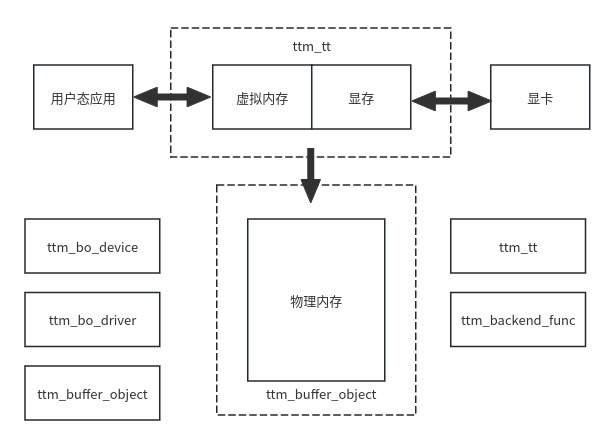
\includegraphics[width=0.8\textwidth]{DRM TTM结构.jpg}
%   \caption{TTM主要对象}
% \end{figure}


\subsection{libdrm接口实现}

\begin{figure}[h]
  \centering
  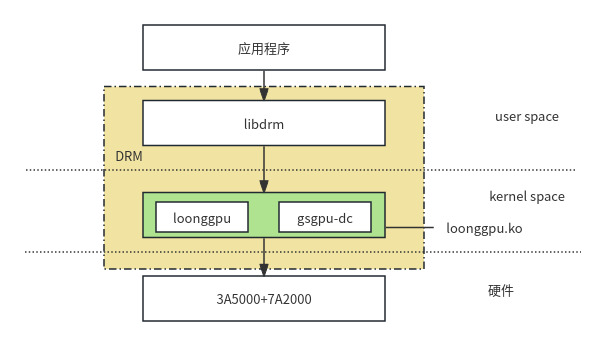
\includegraphics[width=0.8\textwidth]{内核驱动结构图.jpg}
  \caption{内核驱动结构图}
  \label{fig:内核驱动结构图}
\end{figure}

在DRM框架中,libdrm是沟通和连接内核空间和用户空间的重要一环。它通过对多种ioctl底层接口进行封装,以向上提供通用的接口。
用户空间的驱动可以通过libdrm提供的库函数与系统内核进行交互,从而访问底层资源。如图\ref{fig:内核驱动结构图},
libdrm\_gsgpu作为安卓用户空间的驱动程序,它会与底层的DRM内核驱动程序进行通信,
从而完成配置、读取、传输、控制设备等多种行为。

在libdrm中,会通过drmCommandWriteRead封装的读写命令,对内核IOCTL实现进行调用。以gsgpu\_bo\_alloc为例,会在系统内存calloc一块BO缓冲区对象大小的内存,并通过
drmCommandWriteRead封装的args,以DRM\_IOC拆解传入的命令序号作为偏移值,以DRM\_COMMAND\_BASE作为基址获取命令编号,DRM\_IOCTL\_BASE作为操作类型,使用args的大小作为命令数据的大小,
方向默认双向,向内核请求特定的IOCTL操作,随后使用ioctl执行系统调用,操纵DRM设备。libdrm中有关缓冲区对象操作的接口函数如表\ref{tab:libdrmBO接口表},旁边是libdrm函数执行的内核调用的
命令序号,通过上节的IOCTL实现,完成对DRM设备的特定操作。

\begin{table}[h]
  \centering
  \caption{libdrmBO接口表}
  \label{tab:libdrmBO接口表}
  \begin{tabular}{ll}
    \toprule
    libdrm实现  & 命令序号 \\
    \midrule
    gsgpu\_bo\_alloc& DRM\_GSGPU\_GEM\_CREATE  \\
    gsgpu\_bo\_cpu\_map & DRM\_GSGPU\_GEM\_MMAP \\
    gsgpu\_bo\_cpu\_unmap & / \\
    gsgpu\_bo\_export & / \\
    gsgpu\_bo\_free & / \\
    gsgpu\_bo\_import & / \\
    gsgpu\_bo\_list\_create & DRM\_GSGPU\_BO\_LIST \\
    gsgpu\_bo\_list\_destroy & DRM\_GSGPU\_BO\_LIST \\
    gsgpu\_bo\_list\_update & DRM\_GSGPU\_BO\_LIST \\
    gsgpu\_bo\_query\_info & DRM\_GSGPU\_GEM\_OP|DRM\_GSGPU\_GEM\_METADATA \\
    gsgpu\_bo\_set\_metadata & DRM\_GSGPU\_GEM\_METADATA \\
    gsgpu\_bo\_va\_op\_raw & DRM\_GSGPU\_GEM\_VA \\
    gsgpu\_bo\_wait\_for\_idle & DRM\_GSGPU\_GEM\_WAIT\_IDLE \\
    gsgpu\_create\_bo\_from\_user\_mem & DRM\_GSGPU\_GEM\_USERPTR \\
    \bottomrule
  \end{tabular}
  \note{}
\end{table}

\subsection{多版本适配方案设计}
龙芯gsgpu内核驱动属于闭源状态,尚未整合到已有的内核源码,采用的方案为驱动模块独立开发的方式,这样设计有多个方面的好处,

一是为了适应多种方式加载驱动模块的需求,既可以通过加载/lib/modules/\$(kernel\_uname)下
的内核源码头文件实现在已有的系统上动态编译驱动模块并通过DKMS(Dynamic Kernel Module Support)加载,实现在已运行的系统上完成显卡内核驱动模块的安装;也可以通过静态编译,
指定静态的源码树的位置并编译生成可加载的.ko驱动文件。由于安卓主要采用的是静态内核模块(built-in or prebuilt kernel modules)方式来管理驱动,
不支持原生的DKMS,因此本课题采用的是静态编译的方式,在源码树之外编译.ko驱动文件,并在进入安卓系统后使用insmod方式加载.ko驱动文件。

二是为了适应多种内核版本的需求,现龙芯平台主流内核版本为4.19、5.5或6.6,而本课题使用的安卓内核版本为5.10,内核驱动涉及的接口多有变化。
而gpu/drm模块的接口变化较多,这是因为显示模块由于硬件设计上的变化,内核模块的代码需要不断进行调整和优化,以适应现代GPU设备和复杂内存管理的需求。
如表\ref{tab:内核4.19-5.10 drm接口变化}所示,仅从4.19到5.10,drm模块的接口变化已有48项之多,这些接口上的变化导致具体的内核驱动模块需要不断更新迭代,耗时耗力。
因此在原有的4.19内核版本驱动的基础上进行多版本适配,即可以动态识别内核驱动版本接口,是非常有意义的。

\begin{table}[h]
  \centering
  \caption{内核4.19-5.10 drm接口变化}
  \label{tab:内核4.19-5.10 drm接口变化}
  \begin{tabular}{lll}
    \toprule
    类型   &   名称  &变化时内核版本  \\
    \midrule
    变量 & DRIVER\_PRIME & 5.4 \\
    变量 & DRIVER\_IRQ\_SHARED & 5.1 \\
    函数 & drm\_sched\_stop & 5.1 \\
    函数 & drm\_fb\_helper\_fill\_info & 5.2 \\
    变量 & glob(ttm\_bo\_device\_init) & 5.0 \\
    函数 & ttm\_resource\_manager & 5.9 \\
    ... & ... & ... \\
    \bottomrule
  \end{tabular}
  \note{共计48项}
\end{table}

由于drm模块的接口变化为某个函数的增加或删除,部分结构体的属性变化,以及函数的参数变化。以空参数调用某个函数时,若函数相关实现已被删除,则测试代码\textbf{不会产生}编译错误,
仅会在链接时产生错误,而函数存在时,则会产生编译错误,将此种情况命名为function;若某个函数的形参不存在或者结构体或者结构体的某个属性不存在时,则测试代码\textbf{会产生}编译错误,
此种情况命名为type。这两种情况存在和不存在时目标对象时编译结果完全相反,结果判断如表\ref{tab:测试代码判断表}所示。针对不同实现缺失的情形,返回的编译结果完全相反。

\begin{table}[h]
  \centering
  \caption{测试代码判断表}
  \label{tab:测试代码判断表}
  \begin{tabular}{lll}
    \toprule
    类型   &   编译结果 & 函数\&属性\&参数是否存在    \\
    \midrule
    function & 不通过 & 存在 \\
    function & 通过 & 不存在 \\
    type & 通过 & 存在 \\
    type & 不通过 & 不存在 \\
    \bottomrule
  \end{tabular}
\end{table}

具体的方式为实现一个conftest.sh的脚本,假使该目标宏定义为DEF,如算法\ref{algo:algorithm1}所示,通过尝试编译测试代码,测试代码中引入已有的内核头文件,并按以下数种情况实现测试代码:

1.某函数实现删除或增加,假设目标测试函数为funcB,使用一个空返回值空形参的测试函数funcTest并调用无参数的目标函数,可视funcA的返回值情况选择是否设置funcB的返回值,
如算法\ref{algo:algorithm2}所示。

2.某函数实现的形参删除或增加,沿用1假设,添加调用funcB所需的参数,调用funcB并返回,如算法\ref{algo:algorithm3}所示。

3.某结构体的删除或增加,假设目标结构体类型为A,在funcTest中使用A的形参即可,如算法\ref{algo:algorithm4}所示。

4.某结构体中属性的删除或增加,沿用3假设,目标结构体的目标属性为c,使用offsetof(offsetof是一个 C语言的宏,
主要用于计算 结构体成员相对于结构体起始地址的偏移量)测试该结构体是否存在属性c,如算法\ref{algo:algorithm5}所示。

通过编译测试代码的结果(即是否生成中间代码.o文件)以及相应的类型(即function或者type)判断是否存在相关实现,并以此为基础生成相应的宏头文件,为GPU内核驱动的具体实现中提供判断基础。

\begin{algorithm}[h]
  \SetAlgoLined
  ...\;
  将测试代码重定向至conftest.c\;
  尝试编译conftest.c并忽略异常输出\;
  \eIf{存在conftest.o文件}{
    \eIf{类型为function}{
      显示未定义DEF并将其重定向至头文件\;
    }{
      显示已定义DEF并将其重定向至头文件\;
    }
  }{
    \eIf{类型为type}{
      显示已定义DEF并将其重定向至头文件\;
    }{
      显示未定义DEF并将其重定向至头文件\;
    }
  }
  \caption{编译检查测试函数}
  \label{algo:algorithm1}
\end{algorithm}

\begin{minipage}{0.45\textwidth}
  \begin{algorithm}[H]
    \SetAlgoLined
    \KwData{void}
    \KwResult{TypefuncB}
    TypefuncB funcTest(void){\\
      return funcB()\;
        or \;
      funcB()\;
    }
    \caption{测试代码示例1}
    \label{algo:algorithm2}
  \end{algorithm}
\end{minipage}
\hfill
\begin{minipage}{0.45\textwidth}
  \begin{algorithm}[H]
    \SetAlgoLined
    \KwData{arg1,arg2,...}
    \KwResult{TypefuncB}
    TypefuncB funcTest(Type1 arg1,Type2 arg2,...){\\
      return funcB(arg1,arg2,...)\;
    }
    \caption{测试代码示例2}
    \label{algo:algorithm3}
  \end{algorithm}
\end{minipage}

\begin{minipage}{0.45\textwidth}
  \begin{algorithm}[H]
    \SetAlgoLined
    \KwData{TypeA}
    \KwResult{void}
    void funcTest(TypeA a){\\
      return \;
    }
    \caption{测试代码示例3}
    \label{algo:algorithm4}
  \end{algorithm}
\end{minipage}
\hfill
\begin{minipage}{0.45\textwidth}
  \begin{algorithm}[H]
    \SetAlgoLined
    \KwData{void}
    \KwResult{int}
    int funcTest(void){\\
      return offsetof(struct B,c) \;
    }
    \caption{测试代码示例4}
    \label{algo:algorithm5}
  \end{algorithm}
\end{minipage}


\section{GPU用户态驱动缓冲区管理实现}
OpenGL ES的实现基于
% \subsubsection{图形 API 支持}
% 打通GPGPU后端支持Gallium3D的通路,确保 OpenGL 的核心功能集成到龙芯平台,确保API 的正确性。

\subsection{gallium实现及接口}
当前Mesa DRI驱动可以分为两部分,一部分是经典驱动(不基于Gallium3D 框架),另一部分是新的Gallium驱动。 
经典驱动由于采用紧耦合架构设计,存在功能模块化程度较低的局限性,当需要适配新型图形接口标准(如Direct3D/Vulkan)时往往需要进行大量代码重构。
为解决这一技术瓶颈,Gallium3D框架通过构建面向现代GPU硬件特性的通用抽象层,将图形API实现与硬件驱动解耦,使得不同图形接口可在统一架构基础上进行扩展开发。
该框架特别将硬件适配层与操作系统交互模块进行分离设计,通过平台适配模块独立化实现了跨系统兼容能力,显著提升了驱动开发效率和可维护性。目前已经有许多
驱动被移植到伽利略架构上了,包括nouveau(这个是面向NVIDIA的开源驱动),各种radeon驱动,以及一些软件驱动(swrast, llvmpipe)等。
龙芯显卡正是在此架构上实现的。

Gallium Winsys 框架 是 Gallium 驱动框架中的一部分,旨在抽象化硬件和操作系统的差异,提供一个统一的接口来管理底层硬件资源(如缓冲区、上下文、内存等)。
它主要服务于图形硬件驱动和 GPU 资源管理,简化了不同平台之间的图形驱动开发。winsys中的关键操作包括缓冲区管理,内存映射,上下文管理,显示同步等。
由于Android系统实际上是使用的linux内核,所以winsys层的实现还是依赖DRM来管理图形资源和显示。
winsys缓冲区管理接口包括\ref{tab:winsys缓冲区管理接口表}

\begin{table}[h]
  \centering
  \caption{winsys缓冲区管理接口表}
  \label{tab:winsys缓冲区管理接口表}
  \begin{tabular}{ll}
    \toprule
    接口名  & 函数名 \\
    \midrule
    buffer\_create & gsgpu\_bo\_create  \\
    buffer\_map & gsgpu\_bo\_map \\
    buffer\_unmap & gsgpu\_bo\_unmap \\
    buffer\_wait & gsgpu\_bo\_wait \\
    buffer\_set\_metadata & gsgpu\_buffer\_set\_metadata \\
    buffer\_get\_metadata & gsgpu\_buffer\_get\_metadata \\
    buffer\_from\_ptr & gsgpu\_bo\_from\_ptr \\
    buffer\_from\_handle & gsgpu\_bo\_from\_handle \\
    buffer\_get\_handle & gsgpu\_bo\_get\_handle \\
    \bottomrule
  \end{tabular}
  \note{}
\end{table}

\subsection{缓冲区对象(BO)管理}

\subsubsection{显式分配}

如图\ref{fig:gsgpuBoCreate流程图}
首先是参数校验,即在CPU不可访问下还创建VRAM缓冲对象,然后是根据gart\_page\_size对齐内存大小。为了复用缓冲区,避免重复分配内存,尝试从现有的缓冲区缓存池中
获取一个已有的缓冲区。如果缓存未命中,则调用gsgpu\_create\_bo。
gsgpu\_bo\_create首先在系统内存中分配缓冲区对象,并初始化缓存对象的缓存条目,构造缓冲区分配的请求结构,主要是为了区分申请的是VRAM内存还是GTT内存,
之后通过gsgpu\_bo\_alloc(libdrm实现的接口)分配硬件缓冲区;若缓冲区分配成功,则调用gsgpu\_va\_range\_alloc分配虚拟地址空间并设置虚拟地址的内存标志;
调用gsgpu\_bo\_va\_op\_raw映射虚拟地址;若映射成功,则使用缓冲区及相关字段如大小、对齐方式、使用方式、虚拟地址等初始化缓冲区对象,并更新VRAM/gtt的内存统计数据,返回缓冲区对象。
\begin{figure}[h]
  \centering
  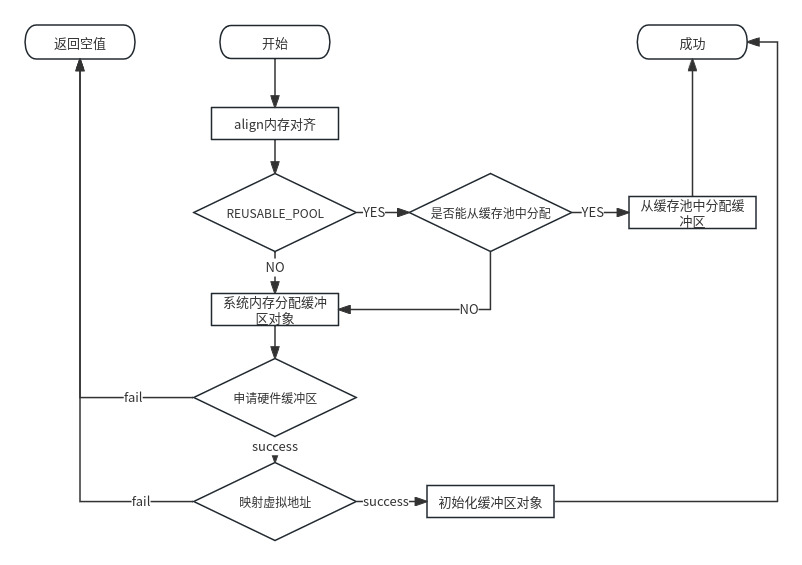
\includegraphics[width=1\textwidth]{gsgpuBoCreate流程图.jpg}
  \caption{gsgpuBoCreate流程图}
  \label{fig:gsgpuBoCreate流程图}
\end{figure}

外部导入:

从共享句柄,为系统导入一个 GPU 缓冲区对象,从而实现对跨进程缓冲区的共享。首先是初始化缓冲区对象,并根据传入的handle句柄类型设置是共享句柄还是DMA缓冲区文件描述符,以设置缓冲区对象的句柄类型。
而后调用gsgpu\_bo\_import导入缓冲区,通过传入的句柄获取缓冲区对象,使用gsgpu\_bo\_query\_info获取大小内存域等信息,并分配虚拟地址空间并映射到缓冲区,这里与显示分配中虚拟地址的分配类似。
在确定缓冲区的初始内存域为VRAM或GTT后,初始化缓冲区对象的字段,并设置步幅和相应的偏移量,更新VRAM/gtt统计数据后返回缓冲区对象。
用户内存映射:

\subsubsection{内存映射与同步}

映射操作:

BO映射重要一步就是缓冲区的同步,在读取纹理数据、动态更新顶点缓冲区等都需要保证数据的一致性。
如图\ref{fig:gsgpuBoMap流程图}
首先是同步检查与处理,如果没有同步的要求,则直接跳转CPU映射操作。如果需要同步访问,可分为阻塞模式和非阻塞模式,在非阻塞模式下,通过检查缓冲区是否被引用判断是否异步刷新命令流。
这里在检查缓冲区引用状态时会稍有区别,当映射可读缓冲区时,若是缓冲区被GPU以读用处占用时,此时并不影响读取的结果,立即检查缓冲区是否可读,若是可读,则可以进行缓冲区的映射操作;
若是缓冲区被GPU以写用处占用时,则会产生冲突需要完成同步操作。若是映射可写缓冲区时,由于写操作会影响缓冲区的读写结果,此时要求缓冲区完全空闲才可以进行缓冲区的映射。
而在阻塞模式下,缓冲区检查与上文类似,但是由于是阻塞模式,会同步刷新命令流,并且在尝试避免忙等待之后会无限期等待缓冲区可读/写。
在CPU映射操作中,会调用libdrm的gsgpu\_bo\_cpu\_map获取CPU的虚拟地址,
若首次映射成功则及时更新mapped\_vram或mapped\_gtt的统计值,并返回映射地址,若失败则释放缓冲区中的所有缓存后重新尝试映射。

\begin{figure}[h]
  \centering
  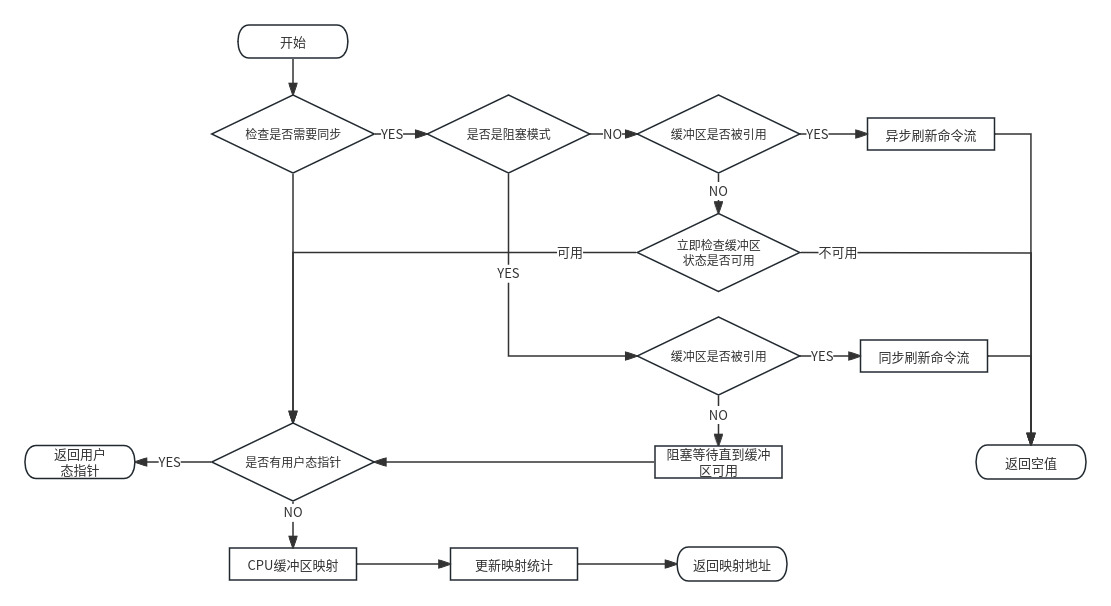
\includegraphics[width=1\textwidth]{gsgpuBoMap流程图.jpg}
  \caption{gsgpuBoMap流程图}
  \label{fig:gsgpuBoMap流程图}
\end{figure}

同步等待:

同步操作就是等待GPU缓冲区完成当前的所有操作。需要确保缓冲区在某些条件下变为闲置或完成特定任务,如等待 GPU 操作结束,或者等待其他进程对缓冲区的操作完成。
根据不同的输入参数(如超时时间、使用类型等)执行相应的等待操作。若超时时间为0,表示立即处理,在此情况下需要先检查缓冲区有无正在进行的IOCTL操作,如果有则表示异常。
而缓冲区若是共享的话,是不能使用用户空间的栅栏(fence)的,需要调用gsgpu\_bo\_wait\_for\_idle等待缓冲区变为空闲之后返回。
之后是等待fence的完成,在立即模式下(即超时时间为0),锁定fence数组,把已经完成的标记从数组里清理掉,更新数组长度;
而若是阻塞模式(即有超时时间),则需要在锁定fence数组后,逐个解锁标记并等待完成,若是超时或者有新的标记添加就停止等待,循环直到所有标记清空或超时。

\subsubsection{跨进程共享}
对应BO管理的外部导入功能。通过获取缓冲区对象的句柄,根据句柄类型赋值type,在调用gsgpu\_bo\_export会根据type执行不同的导出操作,并将句柄储存在输入的结构体中。
之后会标记该缓冲区为共享缓冲区。

% 4.元数据管理 

% BO销毁流程:
% 1. 解映射GPU VA(gsgpu_bo_va_op)
% 2. 释放VA空间(gsgpu_va_range_free)
% 3. 释放硬件缓冲区(gsgpu_bo_free)
% 4. 清理围栏数组(gsgpu_bo_remove_fences)
% 5. 更新内存统计(allocated_vram/gtt)

\section{基于龙芯显卡的安卓图形硬件抽象层实现}

\subsection{硬件混合渲染模块}
%每个厂商hwc实现可能不同如nxp,rockchip,drm-hwc,ranchu,也有很多厂商实现是闭源的如nxp,而谷歌的drm-hwc,ranchu是开源的

\begin{figure}[h]
  \centering
  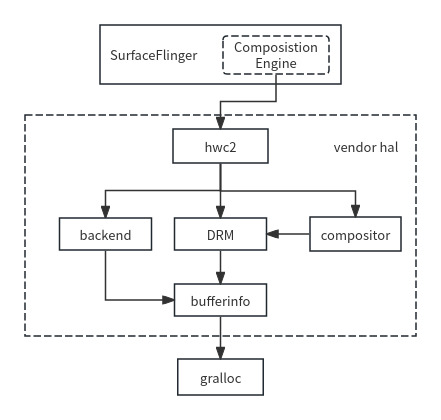
\includegraphics[width=0.8\textwidth]{HWC模块结构.jpg}
  \caption{HWC模块结构}
  \label{fig:HWC模块结构}
\end{figure}

主要模块及实现细节:

1.DRM管理模块
该模块是硬件混合渲染器的核心模块,负责直接与 Linux DRM/KMS(Direct Rendering Manager/Kernel Mode Setting)子系统交互,管理显示硬件资源,
定义了一系列与DRM相关的资源类,如DRM设备抽象、原子提交状态管理、硬件资源对象(Connector/CRTC/Plane/Encoder)、帧缓冲导入等。封装了
原子提交(Atomic Commit)、帧缓冲管理(DrmFbImporter)、资源管理(ResourceManager)、VSync 事件处理(VSyncWorker)、显示管线配置(DrmDisplayPipeline)等一系列功能。

该模块依赖缓冲区信息模块解析图形缓冲区的硬件属性。

2.HWC2接口模块
该模块通过实现HWC2标准定义的接口(如hwc2\_device\_t结构体中的函数指针),将SurfaceFlinger传递的图层数据转化为针对特定显示硬件的合成操作。
其主要工作流程始于Android图形系统的合成请求,通过prepare阶段评估各图层的合成可行性,利用硬件覆盖平面(Overlay Plane)优化性能,避免不必要的GPU参与,
最终在present阶段通过DRM原子提交将配置好的显示帧推送至屏幕。

模块内部通过HwcDisplay类管理单个物理显示设备的状态,包括分辨率、刷新率等显示属性的动态配置,同时处理热插拔事件与多显示器协同工作。
每个图层由HwcLayer对象封装,负责解析Android传递的缓冲区句柄、混合模式及变换矩阵,并通过BufferInfoGetter与底层Gralloc实现交互,获取像素格式、
步长(stride)及DMA-BUF文件描述符等关键元数据。当硬件资源分配时,该模块与合成策略模块(如DrmKmsPlan)协同,决策如何将图层分配到不同的DRM平面
(如Primary Plane用于主图层,Overlay Plane用于视频叠加),并处理缩放、旋转等硬件加速特性。

该模块依赖于后端管理模块、合成器模块以及DRM管理模块

3.合成器模块
该模块主要完成DrmKmsPlan的创建,在创建计划时通过对显示管线中的所有plane(平面)格式判断是否符合上层创建的Layer(图层)的需求,若符合则将设置plane、Layer、zpos(图层的顺序)
等参数并将新的计划加入显示队列。

该模块依赖于DRM管理模块。

4.缓冲区信息适配模块
该模块主要用于获取不同硬件厂商的Gralloc实现,并提供统一接口获取图形缓冲区的元数据。主要使用hw\_get\_module,以GRALLOC\_HARDWARE\_MODULE\_ID(Android中gralloc模块的标识符
)来加载Gralloc模块。

该模块由于是从Android硬件抽象层加载模块,所以不依赖于任何模块

5.后端管理模块
前段接口功能的内部实现,包括验证显示设备的状态、获取客户端图层的范围、检查硬件是否支持特定类型的合成、计算图形操作数计算、需要额外由客户端处理的层范围等,其中较为主要的是实现了
验证显示设备的状态(ValidateDisplay)方法,属于显示验证阶段的核心逻辑,用于决定哪些图层(Layer)可以被硬件直接合成(Overlay),哪些需要回退到 GPU 合成(Client Composition)。

该模块依赖于缓冲区信息适配模块。

实现细节:

1.设备注册与初始化

这一部分的内容主要是DRM管理模块完成,在创建hwcomposer回调时,首先完成对DRM设备资源的初始化,,需要先打开/dev/dri/card*设备文件,
使用drmSetClientCap方法设置DRM客户端能力标志,用于支持通过统一的接口访问和管理所有类型的显示平面,
并启用和指示图形硬件支持原子操作,使用drmGetCap方法检查是否支持framebuffer 修饰符功能。随后获取DRM设备的主控制权,使用drmModeGetResources方法获取DRM设备的资源,
如CRTCs(显示控制器),encoders(编码器),connectors(连接器)并初始化,显示控制器和编码器初始化较为简单,其实就是分别调用drmModeCrtc、drmModeEncoder并储存返回的
指针。而连接器则需要在使用drmModeConnector获取链接器资源后,检查连接器的DPMS(显示电源管理信号)和CRTC\_ID(显示控制器id)是否正常,EDID(扩展显示识别数据)获取显示设备的能力。
在此之后,需要判断连接器是否支持写回(writeback),以及是否支持写回像素格式、framebuffer 的 ID以及输出同步的栅栏指针等这些属性这些都成功后才能储存连接器的指针。
随后使用drmModePlaneRes获取所有的平面(plane),在初始化时获取平面类型(OVERLAY、PRIMARY、CURSOR),并获取一些与显示控制器、帧缓冲、坐标、大小等相关的设置。事实上,由于龙芯
目前的硬件仅支持PRIMARY和CURSOR平面类型,较为简易,在此不再赘述。若上述过程都无异常则初始化成功完成。

2.验证与显示

实际上,hwcomposer的客户端调用是在SurfaceFlinger中,通过显示钩子函数实现对服务端具体功能的调用。
由于龙芯目前的硬件不支持硬件混合渲染,所以SurfaceFlinger的画面合成过程实际上是基于OpenGL ES完成的,是使用client模式合成,仅使用了HWComposer1.0接口标准的软件实现
也就是使用renderengine(课题使用的是支持了龙芯驱动的skia渲染引擎)合成。
这里的client合成是相对于HWC硬件合成而言的,其合成方式是将layer的内容用GPU渲染到缓冲区,然后由缓冲区送显到显示控制器。
其基本过程是首先获取显示设备支持的所有layer,并判断是否支持上层的需求,随后使用CreateComposition尝试创建合成(事实上在后续present送显时也是调用这个函数),若创建成功则更新
像素操作数等统计信息并返回结果。
在CreateComposition时,会初始化渲染管道pipe,按照zpos排列图层并导入帧缓冲区,为图层创建DrmKms计划,并进行画面更新。
它在进行画面更新时实际上会先atomic设置plane的状态,就是调用libdrm的drmModeAtomicAddProperty接口,用于设置显示设备的相关属性,然后atomic向
底层drm系统提交显示信息,也就是调用libdrm的drmModeAtomicCommit接口,更改显示设备的配置,以完成送显的操作。

% 1.HWC合成周期
% \begin{figure}[h]
%   \centering
%   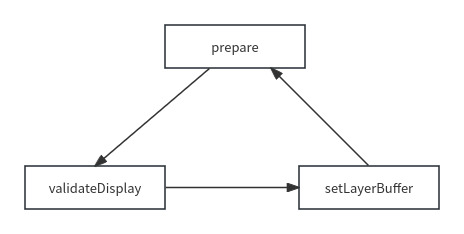
\includegraphics[width=0.8\textwidth]{HWC周期.jpg}
%   \caption{HWC周期}
%   \label{fig:HWC周期}
% \end{figure}

% 准备阶段:
% 每当屏幕内容需要更新时,SurfaceFlinger 会调用 prepare 函数,遍历所有图层并标记它们的合成方式(通过硬件加速device方式还是通过 GPU 合成client方式)。
% 此时会根据图层内容的变化(例如 UI 更新、视频播放等)重新评估每个图层的合成方式
% 验证与提交阶段:
% 在每次显示刷新之前,SurfaceFlinger 会调用 validateDisplay 来检查当前的显示配置是否可以创建DrmKms计划,以检查硬件是否支持。
% 如果硬件支持,则生成 DrmKmsPlan 并准备提交显示计划(调用 presentDisplay提交DRM原子操作)。如果硬件不支持,则回退到 GPU 合成
% 图层提交阶段:
% 在提交图层时,SurfaceFlinger 会使用 setLayerBuffer 更新每个图层的缓冲区,并通过 DrmFbImporter 将 Gralloc Buffer 转换为 DRM Framebuffer。
% 这些 Framebuffer 会被绑定到相应的 DRM Plane,然后将图层显示到屏幕上。

% 2.设备监测
% 显示器热插拔:

% UEventListener 检测到 HDMI 插入 → ResourceManager 重新扫描 Connector → 通知 HWC2 模块更新显示配置。

% 提交显示配置:

% HWC2 调用 DrmAtomicStateManager → 配置 Connector 的 CRTC、Plane 属性 → 提交原子操作。

% 帧缓冲处理:

% DrmFbImporter 将 Android Buffer 转换为 drm\_fb → 绑定到 Plane 的 FB\_ID 属性。


\subsection{图形缓存分配模块}
由于Android系统主要用于arm架构,而arm架构下的GPU多数没有自己的独立显存,系统服务SurfaceFlinger申请的帧缓存属于系统内存,而在本课题中,LoongArch架构下,
GSGPU有自己的专属独立显存。因此首先要解决的是如何让Android的SurfaceFlinger能够在LoongArch架构下运行,而SurfaceFlinger依赖的缓冲区管理的HAL实现就是gralloc。
依照Android 12的gralloc标准,gralloc模块接口定义有两部分,分别是mapper和allocator,
位于AOSP源码结构下的hardware/interface/graphic/mapper以及hardware/interface/graphic/allocator,
其中定义了缓冲区的描述符的数据结构,创建、导入、释放缓冲区对象等。本节按照hal文件定义的接口实现了一个绑定式图形缓存分配器。

gralloc模块的HAL服务有绑定式(Binderized )也有直通式(Passthrough),区别在于,直通式会被编译成.so库文件,为system和vendor分区的进程和应用在运行时动态加载调用,两者是在
同一进程中,而绑定式会被编译成一个可独立运行的服务,类似于一个守护进程,然后相关服务进程或应用会通过HwBinder的IPC(进程间通信)方式来调用,是在两个独立的进程中。绑定式是Google
在Android8.0时,为了方便升级系统框架所做的解耦技术。而绑定式又有默认直通式实现(defaultPassthroughServiceImplementation)以及 注册成服务(RegisterAsService)
两种类型,本课题采用的是第二种。在具体的实现上,采用VINTF Fragments为本模块创建清单并与相应的hal相关联,并且需要设置rc文件并安装到/vendor/etc/init目录下,为init进程初始化
提供执行依据(init进程会在加载init.rc主目录后立即加载/system/etc/init、/vendor/etc/init、/odm/etc/init等相关目录中的文件)。

\begin{figure}[h]
  \centering
  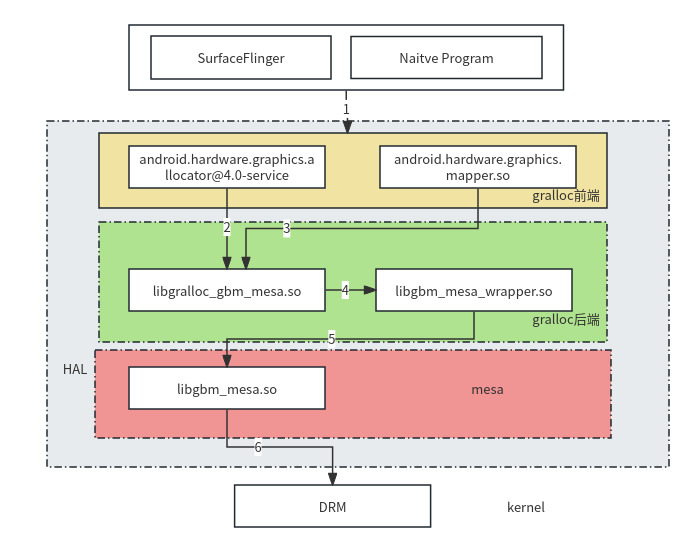
\includegraphics[width=0.8\textwidth]{gralloc调用栈.jpg}
  \caption{gralloc调用栈}
  \label{fig:gralloc调用栈}
\end{figure}

Android自身提供了共享内存的机制,native\_handle\_t是一个用于描述缓冲区的结构体,可以在进程之间传递缓冲区信息,gralloc\_handle\_t是Android 图形缓冲区分配器(Gralloc)中的句柄结构,
它继承自 native\_handle\_t,用于管理共享图形缓冲区。gralloc\_handle\_t这一特性需要libdrm的支持,最低版本需要2.4.97之后才支持此特性,目前龙芯已有的libdrm的解决方案已有2.4.97,
满足相关支持。然后gralloc\_handle\_t图形缓冲区的创建需要显卡驱动的GBM框架(mesa提供的通用缓冲区管理接口)提供支持,然后GBM会调用直接渲染框架(DRI)的接口作为后端,与内核进行交互。
如图\ref{fig:gralloc调用栈}所示,Android系统上层应用程序在需要使用图形缓存时,使用路径1通过IPC(Inter-Process Communication)跨进程通信向gralloc守护进程申请图形缓存,
然后allocator和mapper会通过路径(2-3)调用gralloc后端封装的缓冲区操作函数(函数具体见\ref{tab:gralloc模块后端接口表}),这些操作函数通过路径4调用gbm封装层wrapper,该wrapper封装了
一组与GBM对象操作相关的函数(详细接口见\ref{tab:gbm封装层接口表}),通过路径5直接调用mesa的gbm实现,而gbm会通过路径6内核DRM接口drmIoctl向内核申请创建缓冲区。

\begin{table}[h]  
  \centering
  \caption{gralloc模块后端接口表}
  \label{tab:gralloc模块后端接口表}
  \begin{tabular}{ll}
    \toprule
    接口名  & 作用\\
    \midrule
    init\&close & 驱动程序的初始化和关闭 \\
    bo create & 创建缓冲区对象(BO)的函数,实现内存分配和初始化 \\
    bo destroy & 销毁缓冲区对象的函数,负责释放已分配的内存 \\
    bo import & 导入缓冲区对象的函数,允许将外部缓冲区导入到 GBM 管理的缓冲区中 \\
    bo map & 映射缓冲区对象的函数,使得 CPU 可以访问 GPU 分配的内存 \\
    bo unmap & 解除映射缓冲区对象的函数,释放 CPU 对缓冲区的访问 \\
    bo get plane fd & 获取缓冲区对象平面的文件描述符。\\
    bo get map stride & 获取缓冲区对象的映射跨度。 \\
    resolve format and use flags & 解析格式和使用标志的函数,用于确定缓冲区对象的数据格式及其相关标志 \\
    \bottomrule
  \end{tabular}
  \note{}
\end{table}

\begin{table}[h]  
  \centering
  \caption{gbm封装层接口表}
  \label{tab:gbm封装层接口表}
  \begin{tabular}{ll}
    \toprule
    接口名  & 作用\\
    \midrule
    get gbm format & 获取与设备兼容的 GBM 格式 \\
    dev create/destroy & 创建或销毁 GBM 设备 \\
    alloc & 分配一个 GBM 缓冲区 \\
    import & 导入外部的 GBM 缓冲区 \\
    free & 释放已经分配的 GBM 缓冲区 \\
    map & 将 GBM 缓冲区映射到当前进程的地址空间 \\
    unmap & 解除 GBM 缓冲区的映射 \\
    \bottomrule
  \end{tabular}
  \note{}
\end{table}

\subsubsection{gralloc后端模块}
其中最重要的三个方法就是init、bo create 和bo map,下面将简要描述三个方法的过程。

1.驱动初始化(init)

在驱动程序初始化时,这就需要设置不同的缓冲区格式和使用场景组合。在drv的数据结构中定义了一组向量用于存放定义的缓冲区格式及用途,
可以使用drv\_add\_combinations、drv\_add\_combination 和 drv\_modify\_combination)这几个函数来配置存放的图形驱动的缓冲区管理设置。
具体来说,这些操作是为了为支持不同类型的缓冲区(如扫描输出、纹理、视频编码/解码等)配置不同的格式和元数据。
而常见的缓冲区类型如\ref{tab:缓冲区标志表},这些标志用于标识缓冲区的不同使用场景,通常在图形和视频处理系统中使用。
每个标志代表缓冲区的不同用途,允许驱动程序和硬件根据不同的用途进行优化或操作。

\begin{table}[h]  
  \centering
  \caption{缓冲区标志表}
  \label{tab:缓冲区标志表}
  \begin{tabular}{ll}
    \toprule
    接口名  & 作用\\
    \midrule
    BO\_USE\_NONE & 表示没有任何用途。通常用于初始化或不需要使用标志的情况 \\
    BO\_USE\_SCANOUT & 该标志表示缓冲区将用于显示输出 \\
    BO\_USE\_CURSOR & 该标志表示缓冲区将用于显示光标 \\
    BO\_USE\_RENDERING & 该标志表示缓冲区将用于渲染操作 \\
    BO\_USE\_LINEAR & 该标志表示缓冲区的内存布局是线性的 \\
    BO\_USE\_TEXTURE & 该标志表示缓冲区将作为纹理使用 \\
    ... & ... \\
    \bottomrule
  \end{tabular}
  \note{}
\end{table}

2.缓冲区创建(bo create)

如果是首次创建缓冲区时,需要先初始化并获取一个GbmMesaDriver的实例,使用shared\_ptr存放该实例。在创建时首先需要检查GPU是否需要KMS,
因为一些GPU具有独立的显示控制器,而在龙芯显卡上显示控制器不是独立的。
如果是则需要遍历系统中所有/dev/dri/card*和/dev/dri/renderD*设备节点用于寻找KMS设备,并作为gbm设备节点,如果不是则使用已获取的GPU设备节点作为gbm设备节点。
之后会使用dlopen动态加载libgbm\_mesa\_wrapper.so GBM封装层的动态库,并使用dlsym查找库中的符号GBM\_GET\_OPS\_SYMBOL,该符号会返回一个包含了在gbm封装层接口表中的所有操作的结构体
gbm\_ops。如果成功获取该gbm\_ops,则会调用该接口的dev create方法,以上述寻找的KMS节点文件描述符作为输入创建gbm设备节点作为实际的GBM设备实例。接下来,为 GbmMesaDriver 
创建一个新的私有数据结构 GbmMesaDriverPriv,并将其保存到驱动的 priv 成员中。这样,下一次调用时,函数可以直接获取到已经初始化的 GbmMesaDriver 实例,避免重复初始化。
最后返回 gbm\_mesa\_drv,即创建或已经初始化好的 GbmMesaDriver 实例。
之后设置缓冲区分配参数,gbm即GBM设备,width 和 height即缓冲区的宽度和高度,drm\_format即缓冲区的格式,force\_linear 和 needs\_map\_stride
这些上层调用时传入的 use\_flags设置,指示是否强制使用线性内存布局以及是否需要映射步幅,use\_scanout意思是是否需要扫描输出模式。在处理完无效的drm format格式之后,使用wrapper层的
alloc方法进行缓冲区的分配。之后需要初始化缓冲区布局,为图形缓冲区对象计算和设置与格式相关的属性,如步幅(stride)、大小(size)、偏移量(offset)。
步幅是指从缓冲区中某一行的开始位置到下一行开始位置的字节数。换句话说,它是缓冲区内每行数据的跨度,它告诉我们如何从当前行跳到下一行。
偏移量是指从缓冲区的起始位置到某个数据元素(例如像素、行或平面)的内存地址的距离。它表示数据在缓冲区中的位置。
大小表示缓冲区、图像或某个数据元素所占用的内存空间的大小,通常以字节为单位。

计算步幅需要将原始步幅值stride与目标对齐值stride\_align向上对齐。
\begin{equation}
  stride=(stride+stride\_align-1)\&~(stride\_align-1)
\end{equation}

大小需要步幅乘以平面高度与该平面的垂直子采样因子向上取整。vertical\_subsampling是该平面的垂直子采样因子,表示该平面的高度相对于原始图像高度的缩放比例。

\begin{equation}
  size=((height+vertical\_subsampling-1)/vertical\_subsampling)*stride
\end{equation}

偏移量则是随着对于平面的循环,依次加上大小计算而来。

实际上,由于龙芯目前硬件支持的图形库较为有限,目前使用的硬件平台LG110图层仅支持primary和cursor格式,而不支持layout格式,图像格式上仅支持DRM\_FORMAT\_RGB565,DRM\_FORMAT\_RGB888,
DRM\_FORMAT\_XRGB8888,DRM\_FORMAT\_ARGB8888,cursor仅支持DRM\_FORMAT\_ARGB8888,这些图层的垂直子采样因子皆为1,但是在设计上需要考虑后续对于其他图像格式的支持。
最后创建一个新的私有数据结构 GbmMesaBoPriv,并将其与缓冲区 bo 关联,并设置缓冲区的文件描述符和映射步幅等信息。

在调用wrapper层的alloc方法时,首先初始化alloc\_args作为gbm后端调用的参数,根据输入的参数对width、height进行对齐处理,然后使用wrapper封装的gbm接口,使用gbm\_bo\_create创建
一个新的缓冲区对象bo,以bo作为参数以此调用gbm\_bo\_get\_fd获取缓冲区对象的文件描述符、gbm\_bo\_get\_stride获取缓冲区对象的步长、gbm\_bo\_get\_modifier获取缓冲区对象的格式修饰符,
并在上述步骤完成后可以通过文件描述符对缓冲区进行处理,因此销毁gbm缓冲区对象及时释放资源。gbm中的缓冲区创建等实现实际上是基于直接渲染架构DRI,在创建dri device时,
会搜索目标路径下的所有驱动(本课题使用的是gallium框架实现的驱动)并加载。具体实现会在用户态驱动实现中说明。

% \begin{algorithm}[H]
%   \SetAlgoLined
%   \KwData{gralloc\_buffer\_descriptor,native\_handle\_t}
%   \KwResult{int32\_t}
%   allocate(){\\
%   DRM驱动初始化检查\;
%   ... \\
%   Hal格式与DRM格式检查\;
%   Driver->allocate\;  \tcp{调用驱动的allocate方法} 
%   句柄转换native\_handle\_t 转换成gralloc\_handle\_t\;
%   outHandle设置结果输出\;
%   }
%   \caption{allocate}
%   \label{algo:allocate}
% \end{algorithm}

3.缓冲区映射(bo map)

需要将一个图形缓冲区(bo)映射到用户空间,首先需要通过验证缓冲区的标志,该缓冲区需要有可以被软件访问的标志位,如果没有表示该缓冲区不能映射到用户空间。获取相关的驱动并设置映射的参数,
以获取wrapper层对缓冲区操作的各种函数。在设置完缓冲区映射的大小、缓冲区的格式宽度高度之后,调用wrapper层的map方法来映射缓冲区。该map方法调用gbm\_bo\_map接口,该接口将调用底层
实际的缓冲区映射操作。

\subsubsection{gralloc前端模块}

1.Allocator模块:
由HAL的设计可知,IAllocator中对于allocate方法的定义为
allocate(BufferDescriptor descriptor, uint32\_t count) generates (Error error, uint32\_t stride, vec<handle> buffers);
该方法根据 BufferDescriptor描述符分配指定数量(count)的图形缓冲区,返回原始句柄数组、行步长(stride)及错误状态,其设计需兼顾 硬件适配性、资源管理 及 跨层级数据传递。
方法中的generates表明需要实现一个异步回调接口,descriptor缓冲区描述符是Mappper模块实现的对缓冲区数据结构的序列化后的二进制字节流,基本类型为
uint8\_t。这是安卓为了跨进程传输所设计,也是因为HIDL接口不支持直接传递复杂结构体(如嵌套对象或动态类型),只能支持基本类型和数组。
count是指需要分配的缓冲区数量,数据类型为uint32\_t。在具体的实现时会重载增加hidlCb参数以实现异步回调的功能。算法设计如\ref{algo:allocate}

\begin{algorithm}
  \SetAlgoLined
  \KwData{descriptor,count,hidlCb}
  \KwResult{error,stride,handles}
    \If{mDriver is not initialized}{error $\gets$ Error::NO\_RESOURCES} \tcp{mDriver是支持龙芯驱动的抽象数据结构}
    decode(descriptor) \tcp{反序列化缓冲区描述符} 
    handles.resize(count); \tcp{handles数量扩充至count}
    \For{i:=0 To count-1}{
      loongDescriptor $\gets$ convertDescriptor(descriptor) \tcp{转换数据结构描述符}
      \If{not mDriver.is\_supported(loongDescriptor)}{error $\gets$ Error::UNSUPPORTED}
      ret $\gets$ mDriver.allocate(loongDescriptor,handle)
      \If{ret}{error $\gets$ Error::NO\_RESOURCES}
      error = initialize\_metadata(loongHandle, loongDescriptor)\;
        \If {error != Error::NONE}{
          \tcp{释放当前 handle}
          mDriver.release(nativeHandle)\;
          native\_handle\_close(nativeHandle)\;
          native\_handle\_delete(nativeHandle)\;
          \tcp{回滚:释放已分配的所有 handles}
          \For{j:0 To i}{
              mDriver.release(handle[j].NativeHandle)\;
          }
          return Void()\;
        }
        handles[i] $\gets$ handle\;
    }
      \tcp{回调成功分配的句柄和步长}
      hidlCb(Error::NONE,stride,handles)\;
      \tcp{释放所有的 handles}
      \For{handle in handles}{
        mDriver.release(handle.NativeHandle)\;
      }
      return Void()\;
  \caption{allocate}
  \label{algo:allocate}
\end{algorithm}

其中convertDescriptor是将上层传入的通用描述符转换成龙芯的描述符,由于在安卓的HAL层的DRM\_FORMAT以及缓冲区标志符的命令有所不同,所以需要先进行转换
才能判断对当前缓冲区格式是否支持。可以得出如下的格式转换表\ref{tab:HAL格式转换表}和缓冲区标志转换表\ref{tab:缓冲区标志转换表},
此处仅列出一些常用和目前课题硬件支持的格式。

\begin{table}[H]
  \centering
  \caption{HAL格式转换表}
  \label{tab:HAL格式转换表}
  \begin{tabular}{lll}
    \toprule
    HAL\_PIXEL\_FORMAT & DRM\_FORMAT  & value\\
    \midrule
    HAL\_PIXEL\_FORMAT\_RGBA\_8888 & DRM\_FORMAT\_ABGR8888 & 1\\
    HAL\_PIXEL\_FORMAT\_RGBX\_8888 & DRM\_FORMAT\_XBGR8888 & 2\\
    HAL\_PIXEL\_FORMAT\_RGB\_888 & DRM\_FORMAT\_BGR888 & 3\\
    HAL\_PIXEL\_FORMAT\_RGB\_565 & DRM\_FORMAT\_RGB565 & 4\\
    HAL\_PIXEL\_FORMAT\_BGRA\_8888 & DRM\_FORMAT\_ARGB8888 & 5\\
    ... & ...&...\\ 
    \bottomrule
  \end{tabular}
  \note{}
\end{table}

\begin{table}[H]
  \centering
  \caption{缓冲区标志转换表}
  \label{tab:缓冲区标志转换表}
  \begin{tabular}{ll}
    \toprule
    gralloc\_usage & bo\_use\_flags \\
    \midrule
    GRALLOC\_USAGE\_HW\_COMPOSER & BO\_USE\_SCANOUT | BO\_USE\_TEXTURE \\
    GRALLOC\_USAGE\_HW\_FB & BO\_USE\_NONE \\
    GRALLOC\_USAGE\_HW\_RENDER & BO\_USE\_RENDERING \\
    GRALLOC\_USAGE\_HW\_2D & BO\_USE\_RENDERING \\
    GRALLOC\_USAGE\_HW\_TEXTURE & BO\_USE\_TEXTURE \\
    ... & ...\\ 
    \bottomrule
  \end{tabular}
  \note{}
\end{table}


Mapper模块:同样,IMapper中的方法最主要的是importBuffer、lock、set(实现对元数据的支持)。其中importBuffer方法定义为
importBuffer(handle rawHandle) generates (Error error, pointer buffer);
该方法是将一个原始缓冲区句柄(rawHandle)转换为可在当前进程内安全使用的导入缓冲区句柄。
原始句柄可能来自跨进程传递或克隆操作,直接使用可能存在安全或有效性风险,需通过导入过程生成合法句柄。
在导入过程中需要注意原始句柄的无效性以及错误处理等。算法如\ref{alg:importBuffer}。

\begin{algorithm}
\SetAlgoLined
\KwIn{handle: hidl\_handle}
\KwOut{error: Error, importedHandle: native\_handle\_t}
\If{mDriver is not initialized}{
    \textbf{log error} "Driver uninitialized"\;
    \Return{(Error.NO\_RESOURCES, \text{null})}\;
}
rawHandle $\gets$ handle.getNativeHandle()\;
\If{rawHandle is null \textbf{or} rawHandle.numFds $= 0$}{
    \textbf{log error} "Bad handle"\;
    \Return{(Error.BAD\_BUFFER, \text{null})}\;
}
clonedHandle $\gets$ native\_handle\_clone(rawHandle)\;
\If{clonedHandle is null}{
    \textbf{log error} "Clone failed"\;
    \Return{(Error.NO\_RESOURCES, \text{null})}\;
}
\textbf{Acquire mutex lock}\;
hnd $\gets$ convert\_handle(clonedHandle)\;
\If{hnd is null}{
    \textbf{log error} "Invalid handle format"\;
    \textbf{Release mutex lock}\;
    native\_handle\_close(clonedHandle)\;
    native\_handle\_delete(clonedHandle)\;
    \Return{(Error.BAD\_BUFFER, \text{null})}\;
}
\If{hnd $\in$ handles\_}{
    \tcp{Handle已注册,直接增加引用计数}
    handles\_[hnd].refcount $\gets$ handles\_[hnd].refcount +1\;
    \textbf{Release mutex lock}\;
    \Return{(Error.NONE, clonedHandle)}\;
}
\If{hnd.id $\in$ buffers\_}{
    \tcp{Buffer已存在,增加其引用计数}
    buffer $\gets$ buffers\_[hnd.id]\;
    buffer.refcount $\gets$ buffer.refcount +1\;
}
\Else{
    \tcp{新导入Buffer}
    data $\gets$ populate\_import\_data(hnd)\; \tcp{填充fds/stride等元数据}
    bo $\gets$ drv\_bo\_import(driver, data)\;
    \If{bo is null}{
        \textbf{Release mutex lock}\;
        native\_handle\_close(clonedHandle)\;
        native\_handle\_delete(clonedHandle)\;
        \textbf{log error} "Import failed"\;
        \Return{(Error.NO\_RESOURCES, \text{null})}\;
    }
    buffer $\gets$ create\_cros\_gralloc\_buffer(bo, hnd)\;
    buffers\_[hnd.id] $\gets$ buffer\;
}
\tcp{注册新Handle}
handles\_[hnd] $\gets$ \{buffer, refcount=1\}\;
\textbf{Release mutex lock}\;
\Return{(Error.NONE, clonedHandle)}\;
\caption{importBuffer}\label{alg:importBuffer}
\end{algorithm}

lock方法定义为lock(pointer buffer,uint64\_t cpuUsage,Rect accessRegion,handle acquireFence) generates (Error error,pointer data);
lock 方法用于将图形缓冲区锁定,以便 CPU 直接访问其内存内容。主要用于支持多种访问模式(读/写)和区域限制,并处理并发访问的同步问题。

\subsection{HIDL接口设计与实现}
为了实现绑定式的HAL,需要先根据Android定义的硬件接口规范,使用HIDL语言编写xml文件。编译器会通过该部分的bp文件中定义的vintf\_fragments规则(实际上指向的就是该xml文件),将该
xml文件安装到/vendor/etc/vintf/manifest(系统的安装在/system/etc/vintf/)目录下,在init进程早期阶段通过 VINTF库来加载和解析该目录下的所有HAL实现进行验证并注册。
VINTF 文件中的信息会与设备上已安装的 HAL 实现进行对比以验证 HAL 接口兼容性,在通过 VINTF 文件验证后,Android 会将符合条件的 HAL 接口注册到系统中。
这些接口随后会被 Android 的其他系统服务或应用程序调用。在运行时,VINTF 还负责管理 HAL 接口的动态加载和更新。
通过验证 HAL 接口的版本和兼容性,VINTF 确保系统与硬件设备之间的接口兼容性,避免出现接口不匹配或版本冲突的问题
以Allocator的清单文件为例,使用<manifest>节点作为HIDL文件的起始,
其中version元素的属性表示清单文件的版本号,type表示该清单文件描述的是一个设备类型的 HAL。<hal>节点中的format元素表示该清单描述的是基于 HIDL 的接口,<hal>节点中的
子项name标识了该 HAL 的名称,这是遵循HAL命名空间的约定,表示这是与 Android allocator 相关的 HAL 模块。子项transport表示 HAL 模块使用 hwbinder 作为通信方式。
子项version表示该 HAL 接口的版本号,该版本号为4.0,表示实现的HAL遵循allocator4.0的接口。而<interface>节点中的name元素表示该 HAL 接口的名称是 IAllocator,
是与内存分配器相关的接口,instance元素表示接口的实例名称是 default,通常 HAL 可以有多个实例,但这里指定的是默认实例。而Mapper仅在<transport>子项有所区别,由于Mapper实现的是
直通式,所以是passthrough,且包含arch元素为32+64,表示该接口支持 32 位和 64 位架构。

% 1.gbm包装模块
% 用于在使用 Mesa 和 GBM(Generic Buffer Management)时对显存缓冲区(BO,Buffer Object)进行创建、映射、导入和销毁的操作。它通过封装与 GBM API 的交互,
% 简化了底层内存管理,并与 Android 环境中的驱动配合。实现了以下4个功能模块:
% \textbf{缓冲区分配与管理}:缓冲区可用于多种渲染操作

% \textbf{跨平台支持}:用于纹理处理等操作

% \textbf{优化内存访问}:表示与软件处理相关

% 缓冲区分配与管理: 通过封装 GBM 的创建、导入、映射和销毁操作,实现了对缓冲区对象的管理,方便与其他模块进行交互。

% 跨平台支持: 代码通过不同的条件编译支持在多种架构(如 x86\_64、ARM 等)上的适配,特别是不同平台上缓冲区的对齐和映射步长差异。

% 优化内存访问: 在导入缓冲区时,确保正确的映射步长(map\_stride)处理,避免不同驱动和硬件上的差异,保证高效内存访问。

% 调试与日志: 通过 ALOGE 和 ALOGV 等宏进行调试输出,帮助开发人员调试 GBM 缓冲区分配和管理过程。

% gralloc模块分为HAL服务实现(可以称为gralloc前端),gbm接口实现模块和gbm包装层(可以称为gralloc后端)。前端已有部分开源代码实现,因此可以使用公共层的代码,
% 相应的,本课题只需要实现后端代码,即gbm的接口对接和封装等。

% 由于上层应用是通过gralloc获取实际的图像缓冲描述句柄,而由于不同进程使用图像缓冲区的目的不同。如UI进程是为了渲染画面并传送给SurfaceFlinger进行合成,而SurfaceFlinger是
% 要在自己的缓冲区上合成帧画面并送显,因此图像缓冲区的类型往往不同。

% \textbf{BO\_USE\_RENDER\_MASK}:缓冲区可用于多种渲染操作

% \textbf{BO\_USE\_TEXTURE\_MASK}:用于纹理处理等操作

% \textbf{BO\_USE\_SW\_MASK}:表示与软件处理相关

% \textbf{BO\_USE\_GPU\_HW}:与GPU硬件加速相关

% \textbf{BO\_USE\_NON\_GPU\_HW}:表示与非GPU硬件加速相关

% \textbf{BO\_USE\_HW\_MASK}:表示与所有硬件相关

% 缓冲区对象buffer object数据结构

% drmformat转换、回调框架说明、gralloc直通式等

% 依据硬件的设计可以选择在初始化时是否使用tiled等模式进行访存优化,提供更灵活的驱动交互方式。

% \section{HAL优化}
% 在上述方案实现中,Android gralloc实际上使用的是mesa提供的图形缓冲区管理接口。在3A5000上运行原生的Native程序,如bootanim,

% \subsection{接口优化}
% 在实际的测试中发现由于调用栈过长导致访存成为瓶颈。
% 现重构gbm后端实现以实现对libdrm和DRI驱动的直接调用。

% createImageWithModifiers

% \subsection{tile访存优化}


\section{系统镜像构建}

\subsection{龙芯OpenGL ES驱动构建}

mesa使用的版本为18.3.6,而由于现有的安卓版本为12.0.0,安卓API版本为31对应的mesa版本为20.3.4,因此需要对现有的mesa的dri接口进行升级。并且由于安卓新的
编译方式Soong的加入,mesa目前最新的版本已经废弃了传统的mk编译方式,转而采用伪编译的方式。为考虑后续版本的兼容性,因此在现有的mesa18.3.6上采用伪编译的方法,
使用mesa原生的ninja编译方式,将生成的动态库文件添加到安卓目标生成目录中。此后,mesa库将被编译为libgallium\_dri.so以及libglapi.so。其中libgallium\_dri.so
用于支持DRI使得应用程序可以直接与GPU进行通信,绕过X服务器从而实现更高效的渲染;同时实现多个图形API,包括OpenGL,利用Gallium3D的架构来支持gsgpu的后端。而libglapi.so
则负责管理OpenGL API调用的分发,将调用路由到适当的实现,通常是后端的图形驱动程序并且处理OpenGL上下文的创建、管理和切换,确保正确的状态和资源在不同的渲染上下文中得到维护。
由此背景,可以分析得到以下数个方面。

由于mesa是一个开源的OpengGL实现,提供了多种GPU硬件的驱动支持,因此代码提交量极大。而mesa原生编译框架使用的是ninja,而Android中使用的是Makefile,直接编译生成目标动态库文件,
与原生ninja并无关系,因此需要使用伪编译框架去生成动态库文件,即用cross-compile配置mesa交叉编译脚本aosp-cross,再使用原生ninja编译规则生成目标安装目录install,
将生成的目标文件安装到AOSP编译框架指定的vendor分区,为后续龙芯mesa版本提供支持。

mesa编译框架如图\ref{fig:mesa编译框架},AOSP编译框架会自动监测所有的Android.mk并编译,Android.mk会调用mesa3d\_cross.mk生成aosp\_cross的mesa交叉编译规则,
按照mesa原生的编译规则生成安装目录install,再将目标动态库文件安装到指定的vendor分区。
\begin{figure}[h]
  \centering
  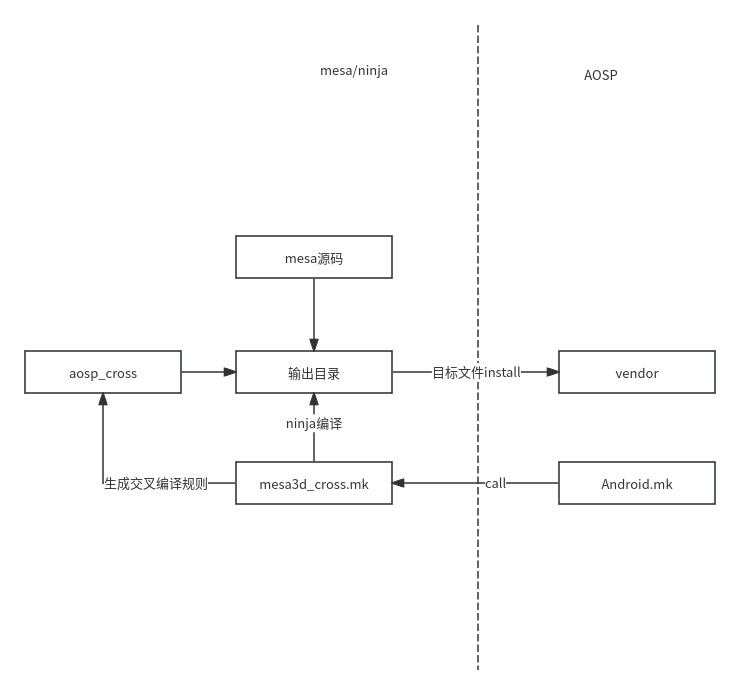
\includegraphics[width=0.8\textwidth]{mesa编译框架.jpg}
  \caption{mesa编译框架}
  \label{fig:mesa编译框架}
\end{figure}

目标安装动态库说明:

libEGL.so.1.0.0,是一个用于处理 EGL (Embedded-System Graphics Library) 接口的共享库,为 OpenGL ES 或 OpenVG 提供了对底层图形设备的抽象;

libGLESv1\_CM.so.1.1.0,是一个用于实现 OpenGL ES 1.x(特别是 OpenGL ES 1.1 和 OpenGL ES 1.0)功能的共享库),负责将 OpenGL ES 1.x 请求转换为 GPU 可执行的指令;

libGLESv2.so.2.0.0,是一个提供 OpenGL ES 2.x 功能的共享库,用于支持 OpenGL ES 2.x(及以上版本)的图形渲染,提供了着色器的支持等;

libglapi.so.0.0.0,提供 OpenGL API 调用 的代理功能,使得 OpenGL 函数调用可以通过动态链接的方式,调用不同的 OpenGL 实现库;

以及为了支持gralloc的功能需要安装的libgbm\_mesa.so.1.0.0,提供GBM(Generic Buffer Management)接口的实现,主要用于管理图形缓冲区;

libgallium\_dri.so,提供了 Gallium 框架下的 Direct Rendering Infrastructure (DRI) 驱动程序实现。

上述数个动态库文件,会被安装到对应的供应商(vendor)分区,以供系统服务(如SurfaceFlinger)等使用。


\subsection{安卓系统镜像定制}
由于龙芯显卡 LG110 的存储管理单元(Memory Management Unit, MMU)采用页式管理来处理 GPU 所使用的内存,
所有内部功能模块均使用虚拟地址。在连接到内部网络之前,这些地址需要经过转换。当前,MMU 设计了三级页表结构,且页大小(page size)为 16KB。
然而,Android 12 尚未支持 16KB 的页大小。这意味着需要对以下几个方面进行修改:

\textbf{Bionic 库}:需要在 Bionic 中调整页面数据结构,以支持 16KB 的页大小。

\textbf{安卓通用内核文件系统}:在内核的文件系统(如ext4、super和f2fs)中添加对 16KB 页大小的支持。

\textbf{AOSP部分系统服务}:在 AOSP 中的部分系统服务中也需添加相应的支持。

具体实现方法是使用内联函数 page\_size() 来获取内核中的页大小,从而实现对多种页面大小的兼容。这种改动将确保龙芯显卡的 MMU 
能够高效地与 Android 系统和应用程序进行集成,提供更好的性能和兼容性。

% \subsection{内核编译\&bionic\&部分系统服务修改说明}

\subsubsection{内核定制}
本课题所使用的内核是安卓通用内核5.10,因此在编译时需要添加安卓特性相关的驱动支持如ASHMEM、BINDERFS、BINDERIPC等。
考虑到需要实现对龙芯显卡的支持,在内核编译时需要将loonggpu/lg100\_cp.bin通过CONFIG\_EXTRA\_FIRMWARE选项指定并使用CONFIG\_EXTRA\_FIRMWARE\_DIR指定固件所在的
位置。由于LG110硬件设计上的限制,因此虚拟内存管理只能使用三级页表,页表大小为16Kb。现需要将内核部分模块做硬件适应性修改,如f2fs模块等,
详见表\ref{tab:f2fs模块修改说明}。以此为基础,对f2fs模块中所有依赖这几个宏的相关实现进行修改。

\begin{table}[h]
  \centering
  \caption{f2fs模块修改说明}
  \label{tab:f2fs模块修改说明}
  \begin{tabular}{lll}
    \toprule
    宏名   &   原有  &改动  \\
    \midrule
    F2FS\_MAX\_LOG\_SECTOR\_SIZE & 12 & PAGE\_SHIFT \\
    F2FS\_LOG\_SECTORS\_PER\_BLOCK & 3 & PAGE\_SHIFT - 9 \\
    F2FS\_BLKSIZE & 4096 & PAGE\_SIZE \\
    F2FS\_BLKSIZE\_BITS & 12 & PAGE\_SHIFT \\
    \bottomrule
  \end{tabular}
  \note{}
\end{table}

\subsubsection{根文件系统定制}
安卓文件系统需要定制的部分可分为bionic和部分系统服务。这两个部分的适配的动机与内核类似,
具体实现可以在bionic/libc/platform/bionic/page.h中实现一个内联page\_size()的函数用以实现从内核
中动态获取页表大小,并以此为适配有使用PAGE\_SIZE为4k相关的服务,累积完成40余处的修改。这个函数实现是用getauxval来获取与进程相关的辅助值(auxiliary vector values),而
辅助向量是内核传递给程序的额外信息,通常是在程序启动时传递给它的,用于提供关于系统环境的各种信息。AT\_PAGESZ就是辅助向量常量之一,用于查询系统的页面大小,如算法\ref{algo:获取内核页面大小}
同时,由于Android12中有大量的系统服务依然在使用PAGE\_SIZE宏,因此对相关系统服务做一些适应性修改在所难免,如图\ref{fig:androidS 16k适配改动图}
\begin{algorithm}[H]
  \SetAlgoLined
  \KwData{void}
  \KwResult{size\_t}
  inline size\_t page\_size(){\\
  \eIf{PAGE\_SIZE已定义}{
    return PAGE\_SIZE\;
  }{
    size = getauxval(AT\_PAGESZ)\\
    return size\;
  }
  }
  \caption{获取内核页面大小}
  \label{algo:获取内核页面大小}
\end{algorithm}

\begin{figure}[h]
  \centering
  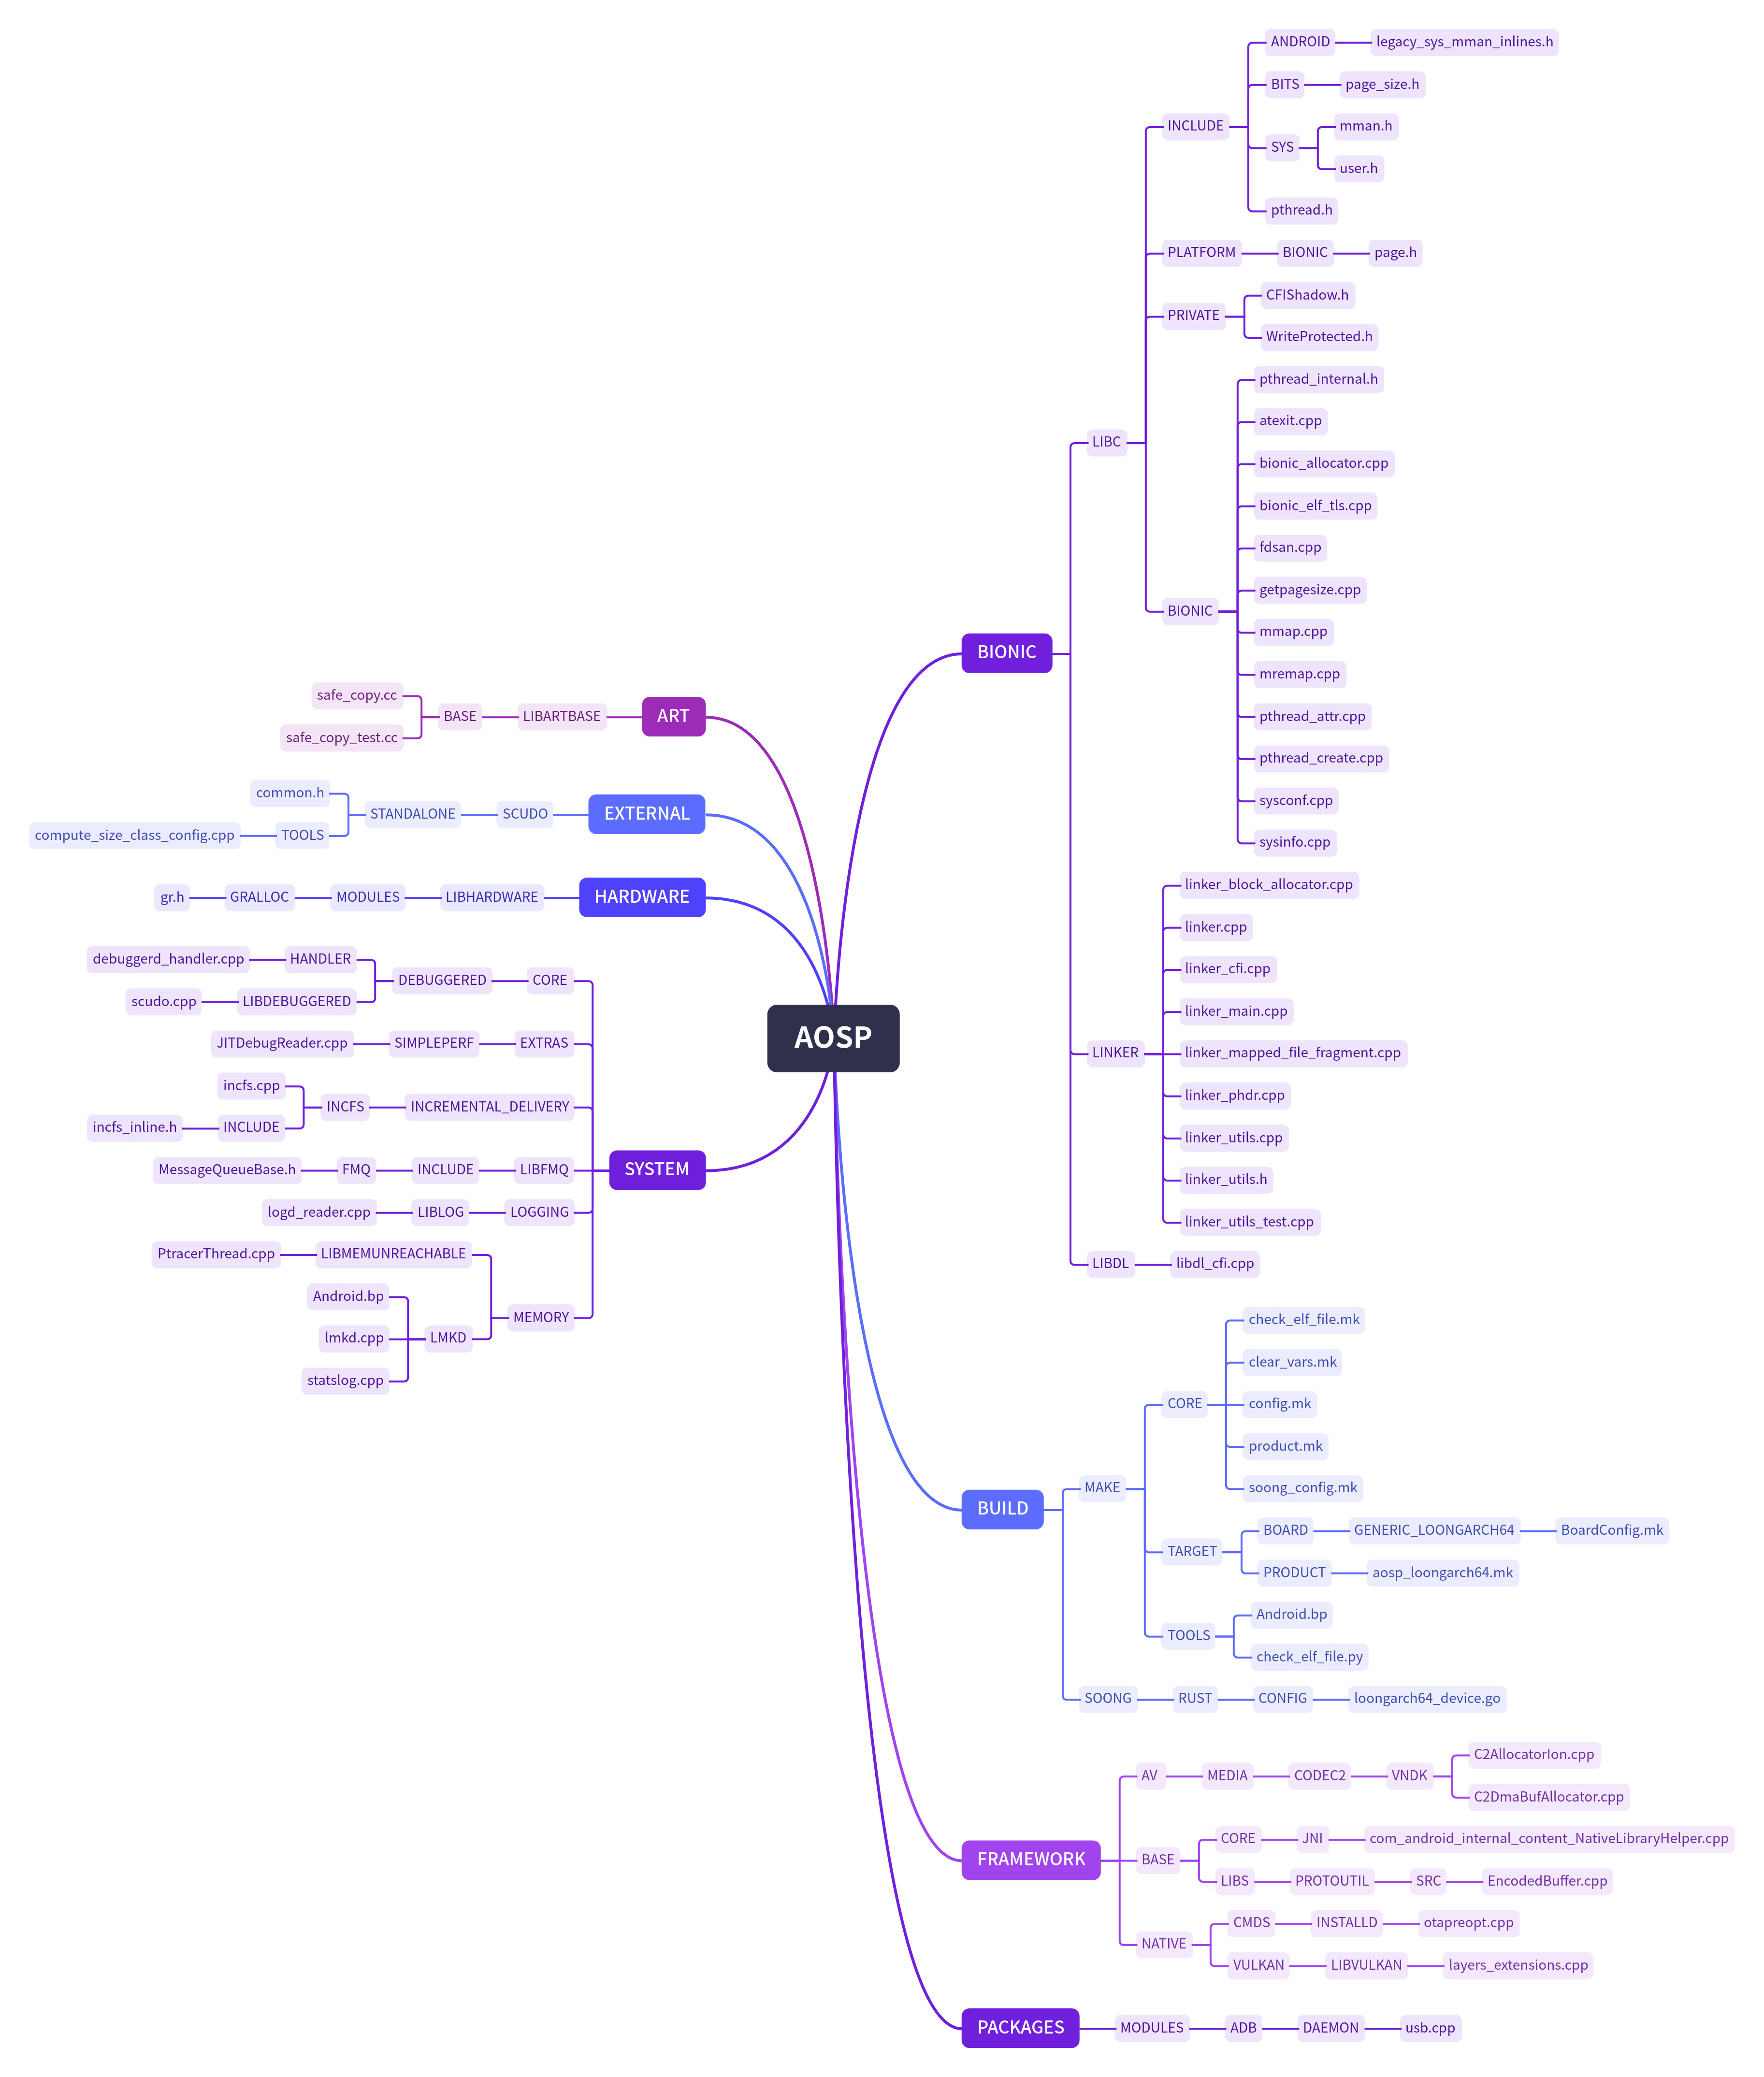
\includegraphics[width=0.8\textwidth]{androidS 16k适配改动图.jpg}
  \caption{龙芯androidS 16k适配改动图}
  \label{fig:androidS 16k适配改动图}
\end{figure}


\section{本章小结}
本章介绍基于龙芯显卡的安卓图形栈的整体设计和具体实现。首先对Android 12的兼容性需求以及HAL接口需求做了分析,然后对图形栈整体的方案做了描述,明确图形栈各组件的实现方案;
接着说明核模DRM和libdrm的ioctl设计接口,以及为了适应内核的多版本需求所实现的一套内核驱动模块多版本适配方案。然后是说明GPU用户态缓冲区管理的实现,并从gallium实现接口和
缓冲区对象管理两个方面说明LG110用户态缓冲区管理是如何实现的。随后从硬件混合渲染模块、图形缓存分配模块以及HIDL接口设计与实现说明基于LG110的安卓图形HAL层是如何实现的。
最后简单说明安卓系统镜像构建方面的需求,包括龙芯OpengGL ES实现的库mesa是如何实现框架外编译,以及因为硬件设计上的缺陷如何对安卓系统镜像进行定制。

% 字段名	对应的函数	功能描述
% name	"gsgpu_common"	模块的名称,通常用于标识该模块或打印调试信息。
% early_init	gsgpu_common_early_init	早期初始化函数,模块初始化前需要做的一些准备工作。
% late_init	gsgpu_common_late_init	后期初始化函数,在其他初始化完成后执行的工作。
% sw_init	gsgpu_common_sw_init	软件部分的初始化函数,通常用于分配内存、初始化数据结构等。
% sw_fini	gsgpu_common_sw_fini	软件部分的清理函数,用于释放资源、销毁数据结构。
% hw_init	gsgpu_common_hw_init	硬件部分的初始化函数,负责配置硬件寄存器或启动硬件功能。
% hw_fini	gsgpu_common_hw_fini	硬件部分的清理函数,负责关闭硬件功能或恢复硬件状态。
% suspend	gsgpu_common_suspend	挂起函数,通常在系统进入睡眠模式(如 S3)时调用,用于保存硬件状态。
% resume	gsgpu_common_resume	恢复函数,通常在系统从睡眠模式恢复时调用,用于恢复硬件状态。
% is_idle	gsgpu_common_is_idle	判断模块是否处于空闲状态的函数,通常用于调试或节能管理。
% wait_for_idle	gsgpu_common_wait_for_idle	等待模块进入空闲状态的函数,通常用于保证操作完成后再进行后续操作。
% soft_reset	gsgpu_common_soft_reset	软复位函数,用于在某些情况下重置模块,而无需对整个系统进行硬复位。
% \subsection{gralloc}

% 1. Allocator
% Allocator 负责内存的分配和释放,主要功能包括:

% 内存分配:
% 分配一块合适大小的内存区域,通常用于图形缓冲区(如帧缓冲、纹理等)。
% 格式支持:
% 支持多种像素格式(如 RGBA、YUV 等),确保分配的内存符合所需的格式和对齐要求。
% 内存管理:
% 管理可用内存的状态,跟踪已分配和未分配的内存区域,确保内存的高效使用。
% 性能优化:
% 通过优化内存分配策略(如缓存机制、批量分配等),提高图形性能。
% 2. Mapper
% Mapper 负责内存的映射和访问,主要功能包括:

% 地址转换:
% 将分配的内存地址转换为应用程序可用的地址,确保应用能够正确访问相应的内存区域。
% 映射和解除映射:
% 提供映射和解除映射的功能,允许应用在需要时将内存映射到其地址空间,使用完毕后解除映射。
% 共享内存管理:
% 支持不同进程之间共享内存,通过 Mapper,多个应用能够高效地访问同一块内存,减少内存复制的开销。
% 权限控制:
% 管理对内存的访问权限,确保只有经过授权的进程能够访问特定的内存区域。

% __DRI_IMAGE_PRIME_LINEAR_BUFFER
% front_rendering_usage __DRI_IMAGE_USE_FRONT_RENDERING 
% 两个扩展新特性可以写一写
% 1. EGL_EXT_image_dma_buf_import
% 功能:允许从 DMA-BUF 导入图像,以实现跨设备的缓冲区共享。
% 应用场景:在多 GPU 系统或使用不同硬件加速的情况下,支持高效的缓冲区共享。
% 2. EGL_ANDROID_image_native_buffer
% 功能:提供对 Android 原生图像缓冲区的支持,允许将图像直接与 Android 的图形系统进行交互。
% 应用场景:用于 SurfaceFlinger、硬件加速的视频播放和图形应用中。
% 3. EGL_ANDROID_surface_texture
% 功能:允许将 SurfaceTexture 用作 EGL 表面,使得 OpenGL ES 能够与 Android 的 SurfaceTexture 直接交互。
% 应用场景:用于实现视频和动画的优化渲染。
% 4. EGL_ANDROID_native_fence_sync
% 功能:支持在图形操作中使用本地栅栏同步机制,以提高 GPU 的并行处理能力。
% 应用场景:在需要同步多个 GPU 操作时提高性能。
% 5. EGL_KHR_create_context
% 功能:允许创建带有特定属性的上下文,增强了对不同版本的 OpenGL ES 的支持。
% 应用场景:为应用程序提供灵活性,以选择合适的 OpenGL ES 版本和功能。
% 6. EGL_EXT_image_gl_colorspace
% 功能:支持不同颜色空间的图像处理,以增强图形的表现力。
% 应用场景:在色彩管理和图像处理应用中使用。
% 7. EGL_KHR_swap_buffers_with_damage
% 功能:允许仅交换需要更新的缓冲区部分,提高交换的效率。
% 应用场景:在需要减少屏幕刷新时提高性能,特别是动态内容的应用。
% 8. EGL_KHR_partial_update
% 功能:支持部分更新 EGL 表面,允许只刷新屏幕的一部分。
% 应用场景:在需要频繁更新部分图像的应用中提高效率



% 安卓的gralloc负责管理图形内存的分配和共享,主要组件包括Allocator,Mapper以及BufferQueue。
% 在API29之后可使用cros grralloc与EGL结合,为gbm(General Buffer Manger)添加支持前渲染的能力。

% 安卓内核编译
%   gsgpu内核驱动编译
% mesa驱动层api兼容方案
% minigbm gsgpu后端接口实现
% 移植兼容方案
%   mesa伪编译代码实现
  %gsgpu内核驱动层多版本兼容方案

% \section{内核态驱动支持}
% gsgpu驱动 ttm,gem,vram
